% STATUS: verified
\chapter{The console and the public site}\label{ch:console}

This chapter shows the system from the screen. It begins with the two web applications that
share the product's address --- the public site, which says what the product is, and the
console, where the work is done --- and with the frame every page of the console sits in:
signing in, the navigation, the two languages, and how a page loads its data, follows a running
job and reports a failure. It then walks through the console page by page, in the order a
person meets the pages, and names for each the chapter that explains the machinery behind it.
The places where the console asks a person to decide are gathered in one table. The public
site and a short account of how the console is built close the chapter.

The screenshots were taken on the console's test data: every company, person, date, amount and
model name in them is made up, and none of them is the live system's. Most are in English; the
console's first language is Lithuanian, and one screenshot shows it so.

\begin{notebox}{The console calls no model}
Neither application calls a language model. The console sends requests to the API (Django) and
to the assistant service, and the assistant service makes every model call (\cref{ch:arch}). What the console does is let a
person start a call --- send a chat message, start an analysis, test a prompt --- and then show
what came back, mark what a model wrote, and offer the place where a person decides. The path
cards of those calls stand in the chapters that own them; \cref{tab:console:modelbuttons} lists
the controls that start one.
\end{notebox}

% ------------------------------------------------------------
\section{Two applications on one origin}\label{sec:console:origin}

One origin serves two single-page applications, built from one Vite project in
\file{vite/app/}. The \term{public site} owns the root of the address (\code{/}): it says
what the product is to a visitor without an account. The \term{console} lives under
\code{/console}: it is the application itself, behind the sign-in. Each has a router of its
own (\file{paths.js}), and a link from one to the other is a plain link that loads the other
application. Both start from one page: the web server in the console's image
(\file{vite/Caddyfile}) answers every address with \file{vite/app/index.html}, and the page's
one script (\file{main.jsx}) starts the console for an address under \code{/console} and the
public site for any other, downloading only the one it starts.

\begin{figure}[H]
\centering
\begin{tikzpicture}
  \node[ext] (browser) at (0,0) {browser};
  \node[svc, text width=24mm] (caddy) at (2.9,0) {static server\\\scriptsize\code{legalops-vite}};
  \node[svc, text width=30mm] (site) at (6.9,1.3) {public site\\\scriptsize\code{/} → \file{site/main.jsx}};
  \node[svc, text width=30mm] (console) at (6.9,-1.3) {console\\\scriptsize\code{/console/*} → \file{console.jsx}};
  \node[chk, text width=30mm] (shared) at (11.6,1.3) {shared: \file{brand.js}, \file{globals.css}, fonts, messages, the \code{locale} cookie};
  \node[svc, text width=27mm] (api) at (11.6,-0.75) {API (Django)\\\scriptsize\code{/api/*}};
  \node[svc, text width=27mm] (asst) at (11.6,-2.15) {assistant service\\\scriptsize\code{/api/assistant/chat}};
  \draw[flow] (browser) -- (caddy);
  \draw[flow] (caddy.north) |- (site.west);
  \draw[flow] (caddy.south) |- (console.west);
  \draw[call] (console.east) -- ++(4mm,0) |- (api.west);
  \draw[call] (console.east) -- ++(4mm,0) |- (asst.west);
  \draw[opt] (site.east) -- (shared.west);
  \draw[opt] (console.north east) -- (shared.south west);
  \node[note, below=0.5mm of site] {asks the backend for nothing};
\end{tikzpicture}
\caption{One origin, two applications. The public site and the console start from the same
page but are separate programs with separate routers; only the console talks to the backend. What they share is the
look and the words: the brand's colours and faces, the stylesheet, the translations and the
cookie that remembers the language.}\label{fig:console:origin}
\end{figure}

\paragraph{Why two applications.} The public site is for a visitor who has no account and
may never sign in. Its start (\file{site/main.jsx}) loads no component library, no query client
and no session, and asks the backend for nothing, so such a visitor never downloads the
console. The console needs all of these. Keeping the two apart lets the public site stay small
and plain while the console carries the weight of a working application.

\paragraph{What they share.} The colours and faces of the brand are one table,
\file{brand.js}: the palette by name (\code{COLORS}), the two font stacks (\code{FONTS}) and
the tints of the four verdict tones (\code{TONES}), with no component library in it. The
console builds its theme from that table (\file{theme.js}); the public site writes the same
values as CSS variables on the page itself (\file{site/main.jsx}). One table means the two
halves cannot drift apart in colour. They also share the stylesheet (\file{globals.css}), the
two self-hosted typefaces, the message files and the \code{locale} cookie, so a visitor who
chose English on the site finds the console in English.

\paragraph{Old addresses.} Until the public site took the root, the console lived there. A
bookmarked report or a link to a conversation from that time now reaches the site's router,
whose catch-all page (\file{site/pages/Missing.jsx}) recognises the console's old first path
segment (\file{site/sitemap.js}) and replaces the address with the same one under
\code{/console}, query and fragment kept. Any other unknown address gets the site's
\enquote{there is no such page}.

% ------------------------------------------------------------
\section{The frame of the console}\label{sec:console:frame}

Every page of the console renders inside the same frame (\file{components/layout/PageLayout.jsx}):
an ink bar on top, the navigation on the left, the page with its title row, and a copyright
band at the end. This section describes what that frame does for every page.

\subsection{Signing in and the session}\label{sec:console:session}

\begin{figure}[htbp]
\centering
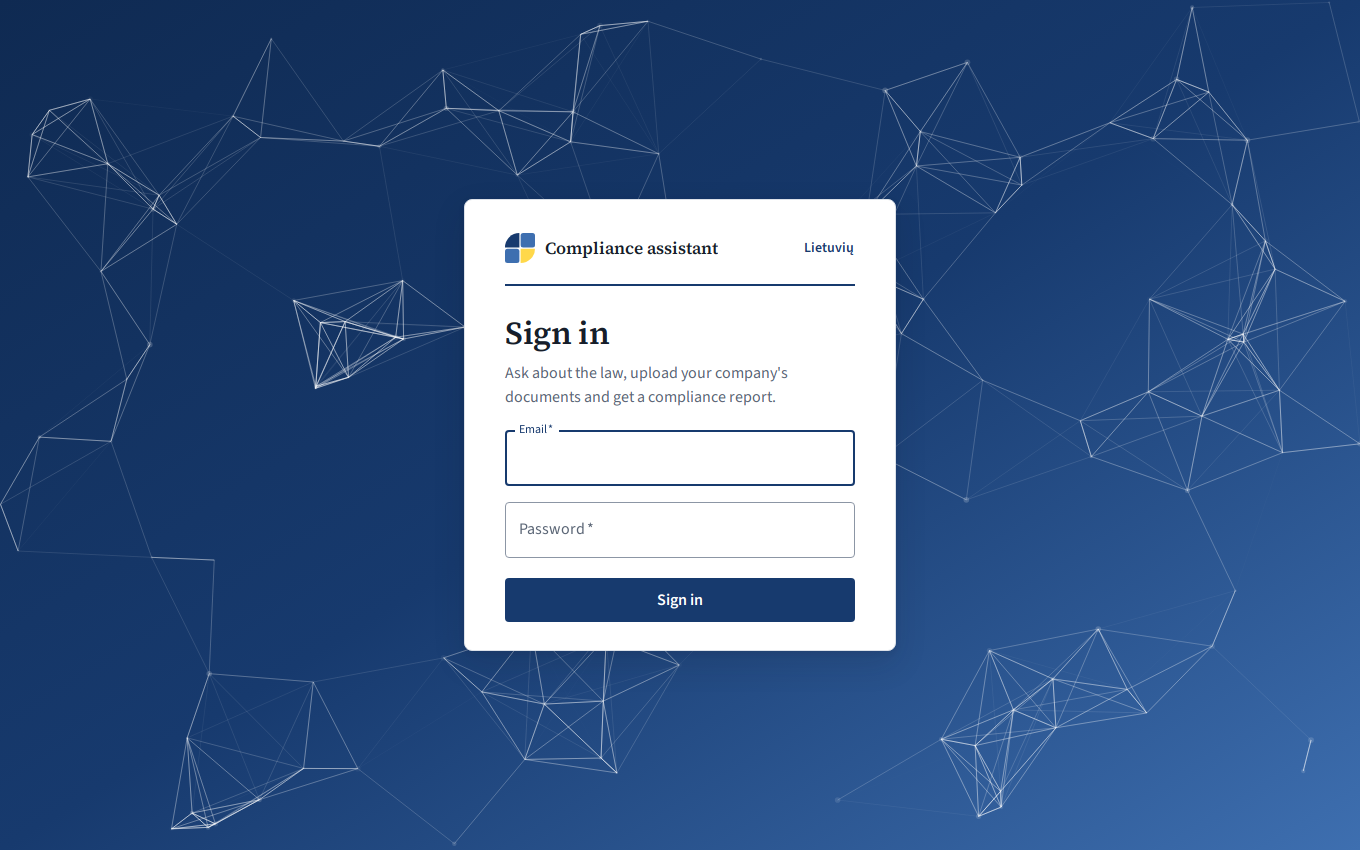
\includegraphics[width=.42\textwidth, trim=440 190 440 190, clip]{figures/screens/login}
\caption{The sign-in page (\code{/console/login}). The wordmark on the sheet links out to the
public site; the language switch sits beside it. Accounts are made by an administrator, so the
page has no sign-up.}\label{fig:console:login}
\end{figure}

The sign-in page (\file{pages/Login/Login.jsx}, \cref{fig:console:login}) asks for an e-mail
address and a password and sends them to \route{POST}{/api/auth/login}. The answer is an opaque
bearer token, which the console keeps in one key of the browser's local storage
(\code{complianceToken}, \file{auth/token.js}) and attaches to every later request
(\file{api/client.js}). The token survives a reload on purpose; the server ends a session after
30 days anyway. The sign-in itself uses a bare request, not the shared client, because a wrong
password is a 401 and must not trigger the client's \enquote{session ended} redirect.

On start the console checks the session once (\route{GET}{/api/auth/me}, \file{AuthGuard.jsx})
and keeps four outcomes apart:

\begin{itemize}
  \item no token at all: straight to the sign-in page, without a request;
  \item a 401, on this or on any later request: the token is dropped and the page is replaced by
    \code{/console/login?next=<here>&expired=1}, which prints \ui{Sesija baigėsi\ldots}
    (\enquote{Your session has ended\ldots}) and, after signing in, returns to where the user
    was;
  \item a server error or a dead network: the token stays, and a full-page card offers a retry
    --- a restart of the backend must not sign everybody out;
  \item an answer that is not an account (an empty body, a page from a misrouted proxy): the
    same card; the console never runs signed in as nobody.
\end{itemize}

The way back in \code{?next=} is honoured only for a path on the same origin
(\file{auth/session.js}, \code{safeNext}), so the parameter cannot be used to send a user to
another site. The account menu in the ink bar holds \ui{Paskyra} (Account) and \ui{Atsijungti}
(Log out); logging out asks the server to end the session and drops the token either way.

\subsection{The navigation, and what each role sees}\label{sec:console:nav}

The navigation (\file{components/layout/Sidebar.jsx}) groups the pages under five titles.
\Cref{tab:console:nav} gives them with their Lithuanian labels, the English beside, and the
role that sees them. A user has one of two roles, \code{user} or \code{admin}. An item marked
for administrators is hidden from a plain user, and the route itself is guarded as well: a
plain user who types such an address gets \enquote{access restricted} inside the normal frame
(\file{PageWrapper.jsx}). The guard is a courtesy, not the protection: the API refuses the data
to a plain user whatever the console shows (\cref{ch:security}).

\begin{table}[H]
\caption{The console's navigation. Paths are given without the \code{/console} base.}\label{tab:console:nav}
\begin{tabularx}{\textwidth}{@{}L{25mm}L{40mm}L{33mm}Y@{}}
\toprule
\hd{Group} & \hd{Item (Lithuanian / English)} & \hd{Path} & \hd{Who} \\
\midrule
\ui{Pagrindinis} Main & \ui{Pokalbis} / Chat & \code{/}, \code{/chat/:threadId} & everyone \\
 & \ui{Apžvalga} / Overview & \code{/dashboard} & everyone \\
\ui{Atitiktis} Compliance & \ui{Įmonės} / Companies & \code{/companies}, \code{/companies/:companyId} & everyone (own companies; an administrator sees all) \\
 & \ui{Ataskaitos} / Reports & \code{/reports}, \code{/reports/:reportId} & everyone (likewise) \\
\ui{Teisė} Law & \ui{Teisės aktų bazė} / Legal corpus & \code{/corpus}, \code{/corpus/:documentId} & everyone reads; administrators also change \\
 & \ui{Pareigų peržiūra} / Obligation review & \code{/obligations} & administrators \\
\ui{Administravimas} Administration & \ui{DI instrukcijos} / AI prompts & \code{/prompts}, \code{/prompts/:slug} & administrators \\
 & \ui{MCP serveriai} / MCP servers & \code{/settings/mcp} & administrators \\
 & \ui{Naudotojai} / Users & \code{/users} & administrators \\
 & \ui{Veiksmų žurnalas} / Audit log & \code{/audit} & administrators \\
\ui{Sistema} System & \ui{DI sąnaudos} / AI usage & \code{/usage} & everyone (own usage; an administrator sees all) \\
 & \ui{Užduotys} / Jobs & \code{/jobs} & everyone (own jobs; an administrator sees all) \\
 & \ui{Paskyra} / Account & \code{/account} & everyone \\
\bottomrule
\end{tabularx}
\end{table}

Two more pages are reached from others rather than from the navigation: the page of one work
product of a compliance programme (\code{/programme/:productId}) and the sign-in page. The
column can be pinned open or folded to a rail of icons that opens over the page when pointed at;
the choice is remembered in the browser. On a phone the navigation is a drawer opened from the
ink bar.

\subsection{Two languages}\label{sec:console:lang}

The console speaks Lithuanian and English, Lithuanian first: it is the default and the
fallback (\file{i18n.jsx}, \code{DEFAULT_LOCALE = 'lt'}). The switch in the ink bar names the
other language (\ui{English} on a Lithuanian page, \ui{Lietuvių} on an English one), changes
the whole interface at once without a reload, and remembers the choice in the \code{locale}
cookie for a year. The page title, the language of the document (\code{<html lang>}) and the
built-in texts of the component library follow it. The language of the interface is not the
language of the content: a report or a work product is written in the language picked when it
is started (which defaults to the interface's), and the chat assistant answers in the language
the user writes in.

\subsection{How a page loads its data and follows a job}\label{sec:console:data}

Every request but the sign-in and the chat's streamed reply goes through one client
(\file{api/client.js}), and every read through one
TanStack Query cache, created in \file{main.jsx} with one retry, so a request that fails twice
shows its error instead of spinning. Pages read; nothing is pushed from the server. Work that
takes long --- an analysis, a generation, the ingestion of an act --- runs as a \term{job} in
the worker (\cref{ch:arch}), and the page that shows it asks again at an interval while the
work is under way, then stops. \Cref{tab:console:polling} lists the intervals.

\begin{table}[H]
\caption{Where the console follows running work, and how often it asks. Each poll stops when the
work has ended; a report that waits for its scope approval is not polled, since only a person
moves it.}\label{tab:console:polling}
\begin{tabularx}{\textwidth}{@{}L{48mm}Yr@{}}
\toprule
\hd{Page} & \hd{Asks while} & \hd{Every} \\
\midrule
One report (\file{ReportDetail.jsx}) & the analysis is queued or running & 3 s \\
Its progress card (\file{ReportProgress.jsx}) & the card is shown (the job's steps) & 3 s \\
Reports list, a company's reports tab & any analysis is queued or running & 5 s \\
A work product's page & the generation is queued or running & 3 s \\
A company's programme tab & any work product is queued or running & 5 s \\
One act of the corpus & its latest job (or the judge's job) is queued or running & 3 s \\
The corpus catalogue & an act is still being ingested & 5 s \\
A company's documents tab & a document uploaded in the last 10 minutes waits for its index & 5 s \\
Chat cards (report, work product) & the analysis or generation runs & 5 s \\
Overview & always (the job queue); the reports while one runs & 10 s \\
Jobs (\code{LIVE_MS}, \code{IDLE_MS}) & anything is queued or running; otherwise & 2 s; 30 s \\
\bottomrule
\end{tabularx}
\end{table}

The worker writes its progress in English (\enquote{3/10 batches}); the console translates
the known messages and turns a job's subject (\code{report:<id>}, \code{corpus:<id>},
\code{product:<id>}) into a label with a link to its page (\file{hooks/useJobText.js}), so that
nothing shaped for a machine reaches the screen.

What a person wants to find again lives in the page's address: the tab, the filters, the
search, the table's page and sort (\file{hooks/useViewParams.js}). A change replaces the
history entry rather than adding one, so Back leaves the page instead of undoing a filter, and
a copied address opens the same view for a colleague; the back link of a detail page returns
to the list as it was left (\file{utils/navigationMemory.js}). A form with unsaved edits asks
before the page is left.

\subsection{Errors and empty lists}\label{sec:console:errors}

A failed read never looks like an empty list. Each section of a page owns its query and, when
it fails, shows a red box with the reason and a retry (\file{components/ErrorState/ErrorState.jsx})
in place of its data; one failed section does not take the others down. A list that loaded
and is empty shows an icon, a sentence and, where there is one, the way forward
(\file{components/EmptyState/EmptyState.jsx}). A failed change (anything but a read) shows a
short notice at the top of the screen; a dialog shows its refusal inside itself instead.

The API answers a failure with an English sentence and a code. The Lithuanian interface must
never show the English sentence or the raw code, so every failure is mapped
(\file{utils/errors.js}): a known code to its own translated sentence, otherwise the HTTP status
to a sentence, otherwise a network or timeout sentence. A rate limit says how long to wait when
the server said so. A page whose code chunk fails to load (a browser tab older than the last
deployment) reloads itself once; only a second failure shows the card saying the application
was updated (\file{pages/RouteError/RouteError.jsx}).

% ------------------------------------------------------------
\section{The tour}\label{sec:console:tour}

The pages follow in the order a person meets them: the chat after signing in, the overview,
the companies and their documents, the reports, what lives on after a report, the programme of
work products, and then the administrator's pages.

\subsection{Chat}\label{sec:console:chat}

\begin{figure}[htbp]
\centering
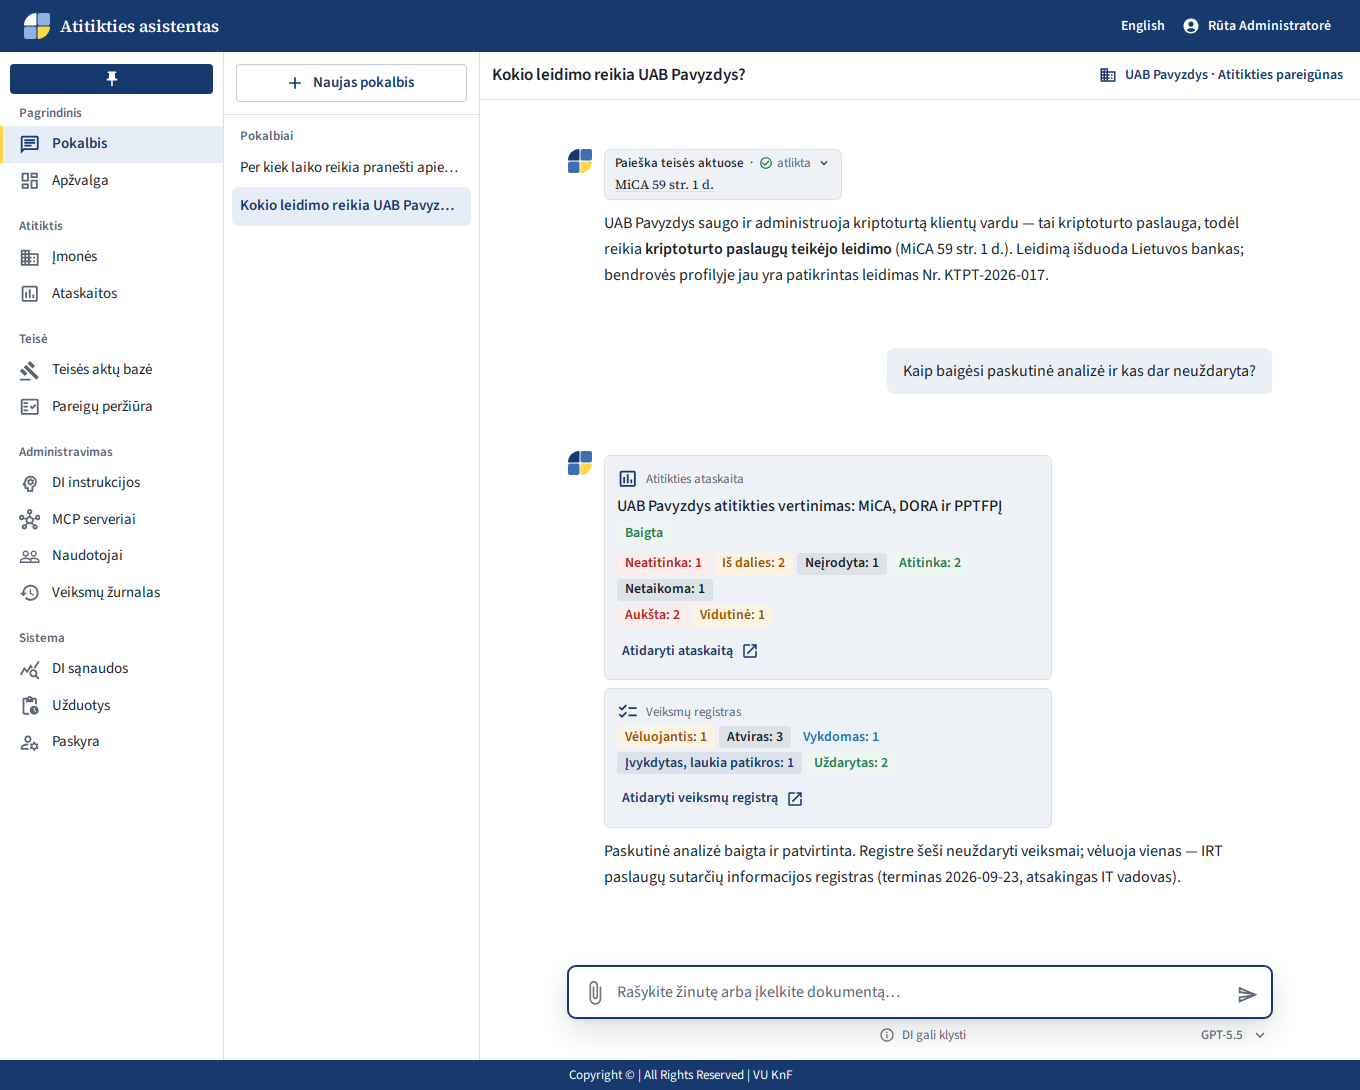
\includegraphics[width=.86\textwidth]{figures/screens/chat-tools-lt}
\caption{The chat in Lithuanian, as an administrator sees it (\code{/console/chat/:threadId}).
On the left the navigation and the conversation list; in the reply, a tool pill
(\ui{Paieška teisės aktuose · atlikta}, \enquote{Searching the legal acts · done}) with the
provision it read, and two tool cards --- a report with its counts and the action register.
In the header, the linked company and role; under the composer, the notice \ui{DI gali klysti}
(\enquote{AI can make mistakes}) and the conversation's model.}\label{fig:console:chat}
\end{figure}

The chat is the console's first page (\file{pages/Chat/Chat.jsx}, \cref{fig:console:chat}).
It has three parts: the conversation list, the thread, and the company panel.

\paragraph{Conversations.} The list holds the user's conversations under
\ui{Naujas pokalbis} (New conversation). A conversation is named from its first message by a
small model (\prompt{chat.title}); a name the user gives it from the pencil on its row is never
replaced. The trash icon removes a conversation from the list after a confirmation; the server
keeps it archived. Coming back to the chat from another page reopens the last conversation;
the chat link inside the chat starts a new one.

\paragraph{The thread.} A message is sent with Enter (Shift+Enter breaks the line). The reply
is written by the assistant service and streamed from \route{POST}{/api/assistant/chat}; it is
written on the server, so closing the page does not lose it, and leaving the page while it is
being written asks first. \ui{Stabdyti atsakymą} (Stop the answer) stops it and keeps what was
written. A reply can be copied or regenerated, a message edited. Replies are model-written
markdown and go through one safe renderer (\file{components/Markdown/Markdown.jsx}): only web
and mail links survive, images become links, raw HTML is shown as text.
Under the field stands a short notice, \ui{DI gali klysti} (AI can make mistakes), whose icon
opens the full transparency text, and on its right the conversation's model: a menu of the
gateway's chat models with their prices, so that a dearer model is a deliberate choice against
the user's daily budget (\file{pages/Chat/ModelPicker.jsx}).

\paragraph{Tool cards.} When the assistant uses a tool, the reply shows it where it was
used (\file{pages/Chat/ToolCards.jsx}). The default is a pill with the tool's name, its state in
words and an icon (\ui{vykdoma…}, \ui{atlikta}, \ui{nepavyko}, \ui{nutraukta} --- running, done,
failed, stopped) and, when opened, the exact input and result; a failed call shows its error
code. Some tools have a card of their own: a corpus search or a citation check lists the
provisions it read, each linked to its official text and, for a check, marked with its verdict;
a cost estimate shows the upper-bound price and the budget left, so the user can answer the
assistant's \enquote{shall I start it?}; a report card shows its status, its live progress and
its counts with a link to the report; a work product card and the action register card do the
same for theirs. A tool of an external MCP server is marked \ui{Išorinis šaltinis} (External
source). The tools themselves are in \cref{app:tools}; the chat's machinery in \cref{ch:chat}.

\paragraph{Files.} A file is dropped onto the composer, pasted, or picked with the paper clip.
It is uploaded at once to \route{POST}{/api/documents} and becomes one of the user's
documents; the chip on the message shows the upload's progress and then the state of its text.
The console refuses before sending a type the system cannot read or a file over 50~MB
(\code{MAX_DOCUMENT_BYTES}, \file{constants/uploads.js}, a copy of the API's limit), and names
the refused file and the reason above the field.

\paragraph{The company panel.} The button in the thread's header names the conversation's
company and role and opens the company panel (\file{pages/Chat/CompanyPanel.jsx}). At its top
the conversation is linked to one of the user's companies (\ui{Susieta įmonė}, Linked company)
and, optionally, to one of that company's role profiles, so the assistant answers from that
role's point of view. Below stand the company's profile, its licences and certificates
(claimed or verified), its documents with the state of their text, its roles, and a link to the
full company page. The panel is read again when a turn ends, since the assistant may just have
created or changed the company through its tools.

\subsection{Overview}\label{sec:console:overview}

\ui{Apžvalga} (Overview, \file{pages/Dashboard/Dashboard.jsx})
answers \enquote{what needs attention}: a row of counts (companies, finished reports, running
analyses with those awaiting scope approval, legal acts ready out of all; for an administrator
also the obligations waiting for review and the users), today's AI budget as a meter, the
latest reports and companies, the health of the corpus with the acts whose ingestion failed,
and the job queue with its queued, running and failed counts, each a link to the jobs page
filtered to that status. Every card loads and fails on its own.

\subsection{Companies}\label{sec:console:companies}

\ui{Įmonės} (Companies, \file{pages/Companies/Companies.jsx}) lists the user's companies; an
administrator sees everybody's with the owner's name and can narrow to their own with
\ui{Tik mano} (Only mine). The search runs on the server over the name and the registration
code. \ui{Nauja įmonė} (New company) creates a profile with its name, code, institution type
and country; the rest is filled on the company's page or by the assistant in the chat.

\begin{figure}[htbp]
\centering
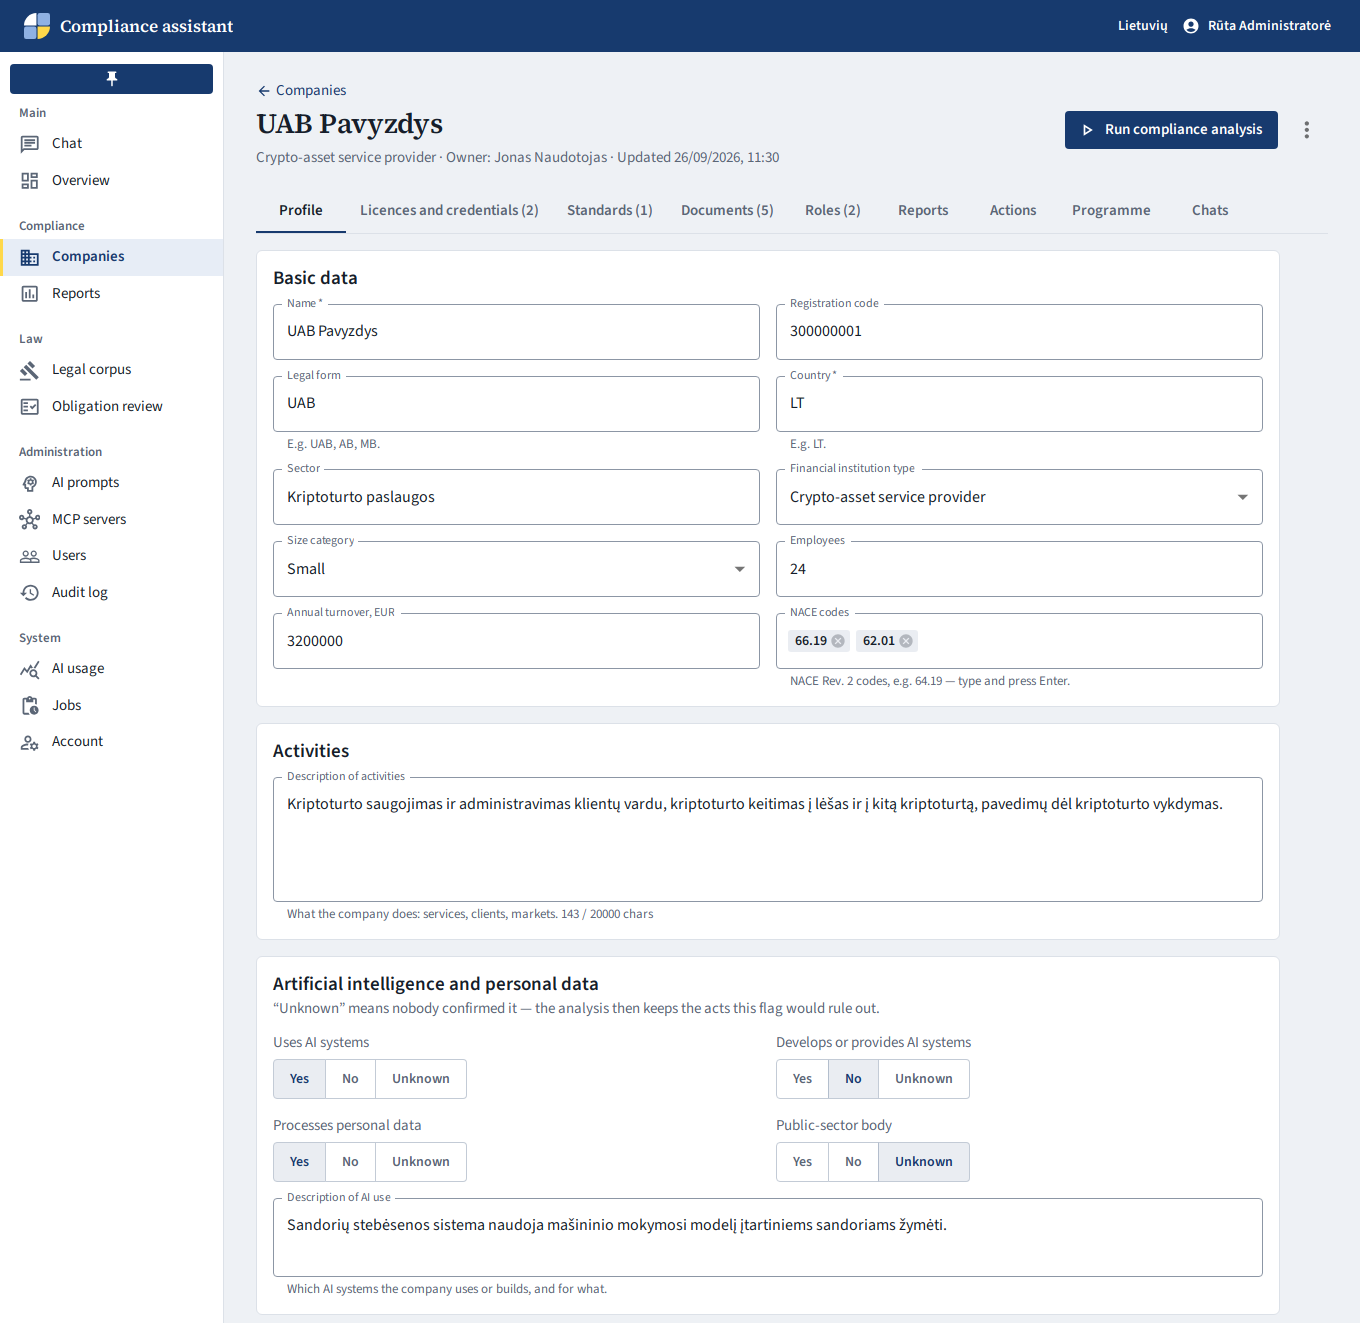
\includegraphics[width=.76\textwidth, trim=240 613 0 52, clip]{figures/screens/company-profile}
\caption{A company's page, profile tab (\code{/console/companies/:companyId}), its top part.
Note the nine tabs with the counts in their names, \ui{Run compliance analysis} in the header,
and the owner's name in the subtitle, which an administrator sees.}\label{fig:console:company}
\end{figure}

A company's page (\file{pages/Companies/CompanyDetail.jsx}, \cref{fig:console:company}) has
nine tabs, listed in \cref{tab:console:companytabs}. The tab is kept in the address
(\code{?tab=}), and a tab once opened stays mounted, so unsaved profile edits survive a look at
another tab. The header carries \ui{Pradėti atitikties analizę} (Run compliance analysis) and a
menu with \ui{Naujas pokalbis apie įmonę} (New chat about the company) and
\ui{Ištrinti įmonę} (Delete the company); a company cannot be deleted while one of its analyses
runs. On a phone-width screen the strip of nine tabs scrolls, and a tab opened by a deep link
can sit under the scroll arrow.

\begin{table}[H]
\caption{The nine tabs of a company's page (\code{TABS} in \file{CompanyDetail.jsx}), in their
order.}\label{tab:console:companytabs}
\begin{tabularx}{\textwidth}{@{}L{38mm}YL{19mm}@{}}
\toprule
\hd{Tab} & \hd{What it shows and what a person can do} & \hd{Machinery} \\
\midrule
\ui{Profilis} Profile & Every field of the profile in cards: basic data, activities, AI and
personal data, the financial-market classification (the assistant's, read-only), additional
data as JSON. The four facts --- uses AI, provides AI, processes personal data, public-sector
body --- are yes / no / unknown; \enquote{unknown} is sent as \code{null}, never guessed, and keeps the acts it
would rule out in the analysis. Saved with one request carrying only the changed fields. &
\cref{ch:company} \\
\ui{Leidimai ir licencijos} Licences and credentials & Licences, permits, registrations,
certificates, each \ui{Deklaruota} (claimed) or \ui{Patikrinta} (verified).
\ui{Pažymėti patikrintu} (Mark as verified) is a confirmed act that records who and when. &
\cref{ch:company} \\
\ui{Standartai} Standards & The standards the company is certified to, implementing or planning,
picked from the standards in the corpus; every later analysis assesses them. &
\cref{ch:company,ch:report} \\
\ui{Dokumentai} Documents & The upload area (kind of document, drop zone), the search over the
documents' text, and the list with the state of the text, of the index and the inventory's
summary. A row opens the document drawer. & \cref{ch:company} \\
\ui{Rolės} Roles & Role profiles a conversation can adopt: a name, a role context of at most
6,000 characters, and its sources in the company's documents. & \cref{ch:chat} \\
\ui{Ataskaitos} Reports & The company's analyses, as on the reports page. & \cref{ch:report} \\
\ui{Veiksmai} Actions & The action register and, under it, the changes in the law
(\cref{sec:console:register}). & \cref{ch:register} \\
\ui{Programa} Programme & The three work products of the compliance programme
(\cref{sec:console:programme}). & \cref{ch:programme} \\
\ui{Pokalbiai} Chats & The caller's own conversations about this company, each a link into the
chat. & \cref{ch:chat} \\
\bottomrule
\end{tabularx}
\end{table}

\paragraph{Documents and the document drawer.} A document is uploaded into the documents tab:
the kind is picked first (policy, procedure, contract, register, other), then files are dropped
or chosen; each goes up with its own progress bar. The text is extracted during the upload and
the index is built by the worker afterwards, which is why the list asks again for a while. The
search box runs the semantic search over the company's documents on Enter only, because every
search embeds the query and costs a little; a hit opens the document at its passage.

When a batch is through, the tab hands its documents to the assistant
(\file{pages/Companies/useDocumentIntake.js}): it opens a conversation of the company
(\route{POST}{/api/chat/threads}) and sends one turn in the user's name
(\route{POST}{/api/assistant/chat}) with the documents that have text attached --- at most 29
a turn, since a message carries 30 parts. What is uploaded while that turn runs waits, and
then goes into a conversation of its own, so that no turn pays for reading the earlier
documents again. Nobody has to ask for anything: the first rule of the chat's prompt has the
assistant read the documents and file what they establish --- the profile, each document's
kind, licences, standards, role profiles (\cref{ch:chat}). A notice under the drop zone says
that the assistant is reading and what it fills in, links to the conversation, and says how
the turn ended: done, or not finished, with the chat's own sentence for the reason (today's
budget spent, no assistant configured, an answer cut short). The conversation of a turn
refused before it began holds nothing and is archived again. The turn runs on the server
and outlives the page.

\begin{figure}[htbp]
\centering
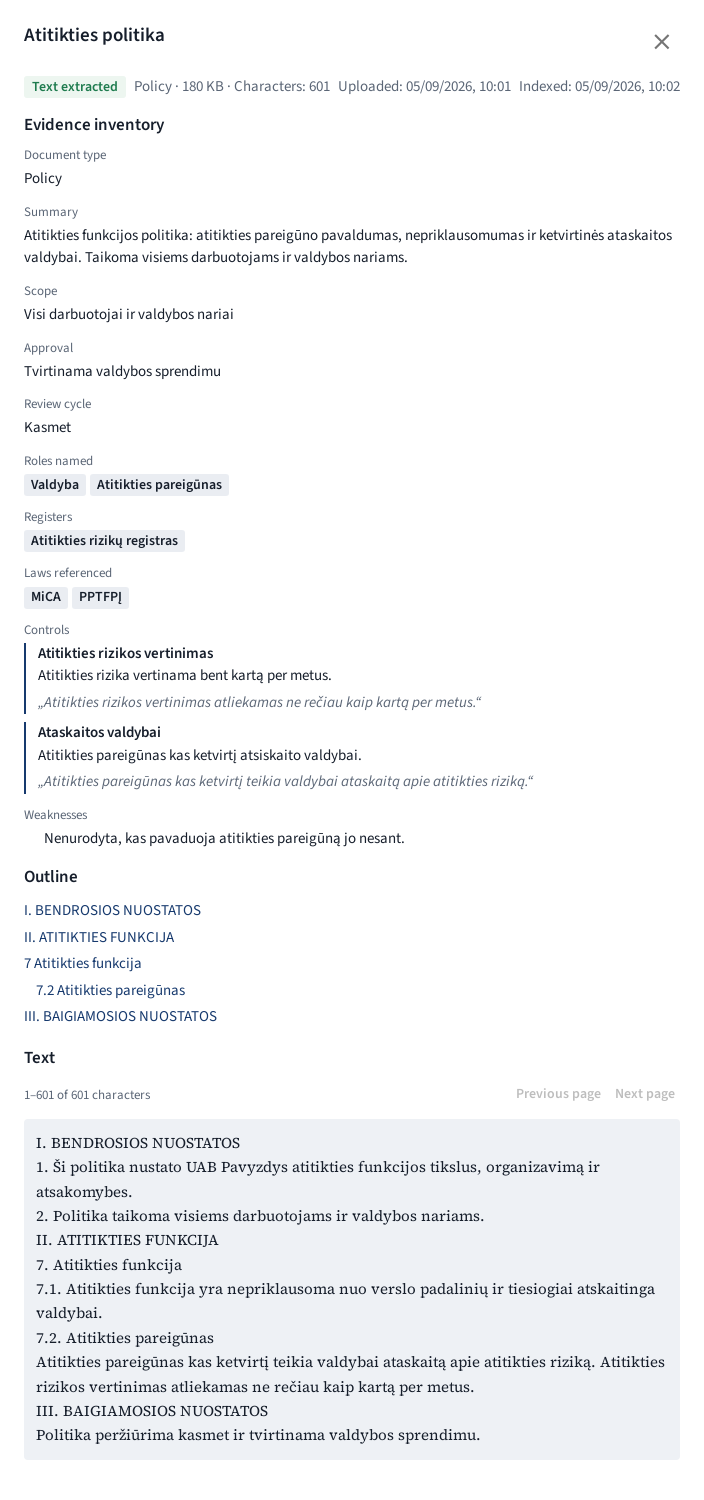
\includegraphics[width=.50\textwidth, trim=0 640 0 0, clip]{figures/screens/document-drawer}
\caption{The top of the document drawer: the state of the text and the evidence inventory a
model read out of the document --- the controls with their quotes, the roles, registers and laws
it names, its weaknesses. The outline and the paged text follow below.}\label{fig:console:drawer}
\end{figure}

The \term{document drawer} (\file{pages/Companies/DocumentDrawer.jsx}, \cref{fig:console:drawer})
is the one place a company document is read in the console. It shows the document's inventory
--- what an analysis read out of it, built once and cached (\cref{ch:company}) --- its outline,
whose headings jump to their place, and its text in windows of 20,000 characters
(\code{TEXT_WINDOW}). The drawer is also where a finding's evidence leads: opened from a
quotation, it shows the page of the text that holds it with the quoted passage under the
yellow marker, so a reader can see the sentence the model relied on in its context.

\subsection{Reports}\label{sec:console:reports}

\ui{Ataskaitos} (Reports, \file{pages/Reports/Reports.jsx}) lists the analyses of the user's
companies (an administrator's: all), filtered by company and by status. A report's status is
one of \ui{Laukia eilėje} (Queued), \ui{Vykdoma} (Running), \ui{Laukia apimties patvirtinimo}
(Awaiting scope approval), \ui{Baigta} (Finished), \ui{Nepavyko} (Failed) and \ui{Atšaukta}
(Cancelled). \ui{Nauja analizė} (New analysis) opens the start dialog with a company picker;
from a company's page the company is fixed. What the analysis does is \cref{ch:report}; here is
what the person sees of it.

\begin{figure}[H]
\centering
\begin{tikzpicture}[node distance=5mm and 7mm, every node/.append style={text width=27mm}]
  \node[man] (start) {start\\\scriptsize consent to the estimate};
  \node[ai, right=of start] (p1) {first part runs\\\scriptsize progress card};
  \node[man, right=of p1] (scope) {scope review\\\scriptsize switches, approve};
  \node[ai, right=of scope] (p2) {second part runs\\\scriptsize progress card};
  \node[svc, below=9mm of p2] (done) {finished\\\scriptsize six tabs, exports};
  \node[man, left=of done] (review) {review findings\\\scriptsize override, cause};
  \node[man, left=of review] (sign) {sign-off\\\scriptsize or withdraw};
  \node[svc, left=of sign] (reg) {action register\\\scriptsize the plan comes in};
  \draw[flow] (start) -- (p1);
  \draw[flow] (p1) -- (scope);
  \draw[flow] (scope) -- (p2);
  \draw[flow] (p2) -- (done);
  \draw[flow] (done) -- (review);
  \draw[flow] (review) -- (sign);
  \draw[flow] (sign) -- (reg);
  \draw[opt] (p1.north) -- ++(0,4mm) -| node[lbl, pos=.25]{without the review} (p2.north);
\end{tikzpicture}
\actorlegend
\caption{A report's page through its life, as the console shows it. The analysis stops after
the first, cheap part and waits for a person to approve the list of acts, unless it was started
without the review (dotted). A finished report is reviewed and signed off by a person; the
sign-off moves the company's action register. The model calls inside the two running parts are
\cref{ch:report}'s.}\label{fig:console:reportlife}
\end{figure}

\paragraph{Starting an analysis.} The start dialog (\file{pages/Reports/StartAnalysisDialog.jsx},
\cref{fig:console:start}) takes the report's language, an optional scope (\ui{Tik šie teisės
aktai (neprivaloma)}, Only these legal acts), and two options. \ui{Įvertinti ir įmonės vidaus
reikalavimų laikymąsi} (Also assess the company's own requirements) adds the check of whether
the company's procedures carry out what its own policies require; it is off, with the reason,
when the company has no policy-level documents. \ui{Tęsti nelaukiant aktų sąrašo patvirtinimo}
(Continue without waiting for the list of acts to be approved) runs the analysis through
without the scope review; left unticked, the analysis stops once it has decided which acts
apply.

\begin{figure}[htbp]
\centering
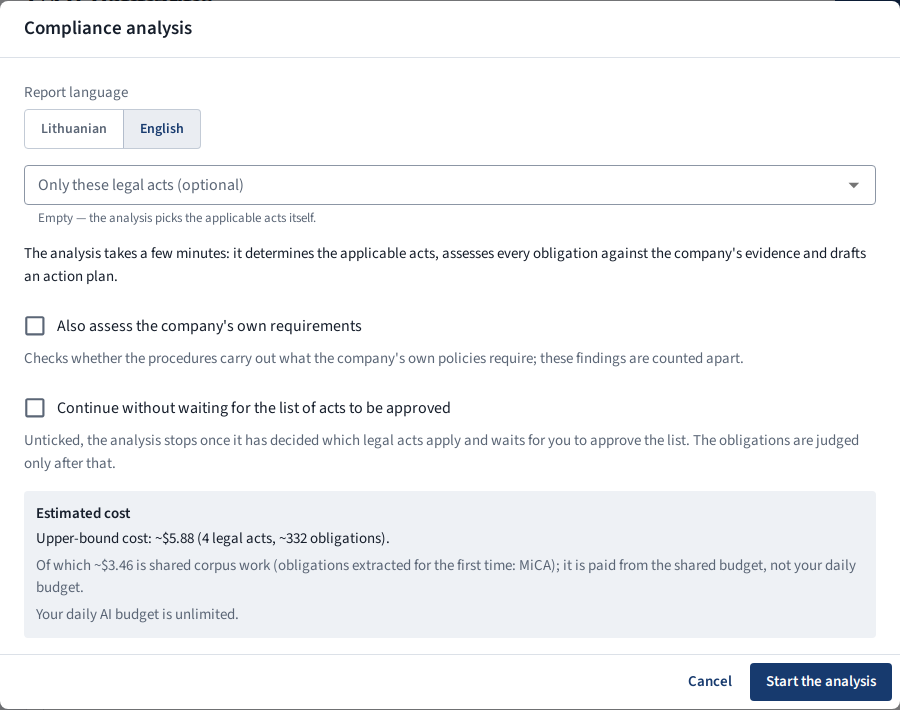
\includegraphics[width=.58\textwidth]{figures/screens/analysis-start-dialog}
\caption{The start dialog. Under the options stands the estimate from
\route{GET}{/api/reports/estimate}: the upper-bound cost with the number of acts and
obligations, the part that is one-time corpus work paid from the shared budget, and the user's
daily budget.}\label{fig:console:start}
\end{figure}

Before the person confirms, the dialog asks the API for an estimate and shows the
\emph{upper-bound} cost of the run, how many acts and obligations it covers, how much of it is
one-time work on the corpus (obligations extracted for the first time), which is paid from the
shared budget and not the user's, and the user's remaining daily budget. When a model's price is
unknown the figure is a floor and says \enquote{at least}. An estimate over the remaining budget
draws a warning but does not block: the API refuses a start only when the day's budget is
almost spent, and a started run is never stopped halfway. The dialog shows the API's three
refusals inside itself, translated: an empty corpus, an analysis of this company already running
or waiting (with a link to it), and a spent budget. How the estimate is computed is
\cref{ch:report}; the budget is \cref{ch:models}.

\paragraph{The scope screen.} A report started with the review stops in
\ui{Laukia apimties patvirtinimo} (Awaiting scope approval). Its page then opens on the
\ui{Teisės aktai} (Legal acts) tab, which becomes the approval screen
(\file{pages/Reports/ReportScope.jsx}, \cref{fig:console:scope}). The acts stand in the groups
the run put them in, each card with the model's verdict, confidence, reasoning and the scope
provisions it cited, and an \ui{Vertinti} (Assess) switch that starts where the run decided.
Switching an act on that does not bind the company assesses it as good practice; switching an
applicable act off leaves it out; the card says so in words. Every move of a switch asks the API,
after a short pause, for the price of the second part for that selection (the same
\route{POST}{/api/reports/{id}/scope} without \code{approved}, which stores nothing).
\ui{Patvirtinti ir tęsti} (Approve and continue) sends the decision with \code{approved: true}
and the run continues; \ui{Atšaukti analizę} (Cancel the analysis) ends it. The switches are
kept in the browser tab while the person looks elsewhere. The report and its exports later name
who approved the list and when, and set apart the acts decided against the verdict.

\begin{figure}[htbp]
\centering
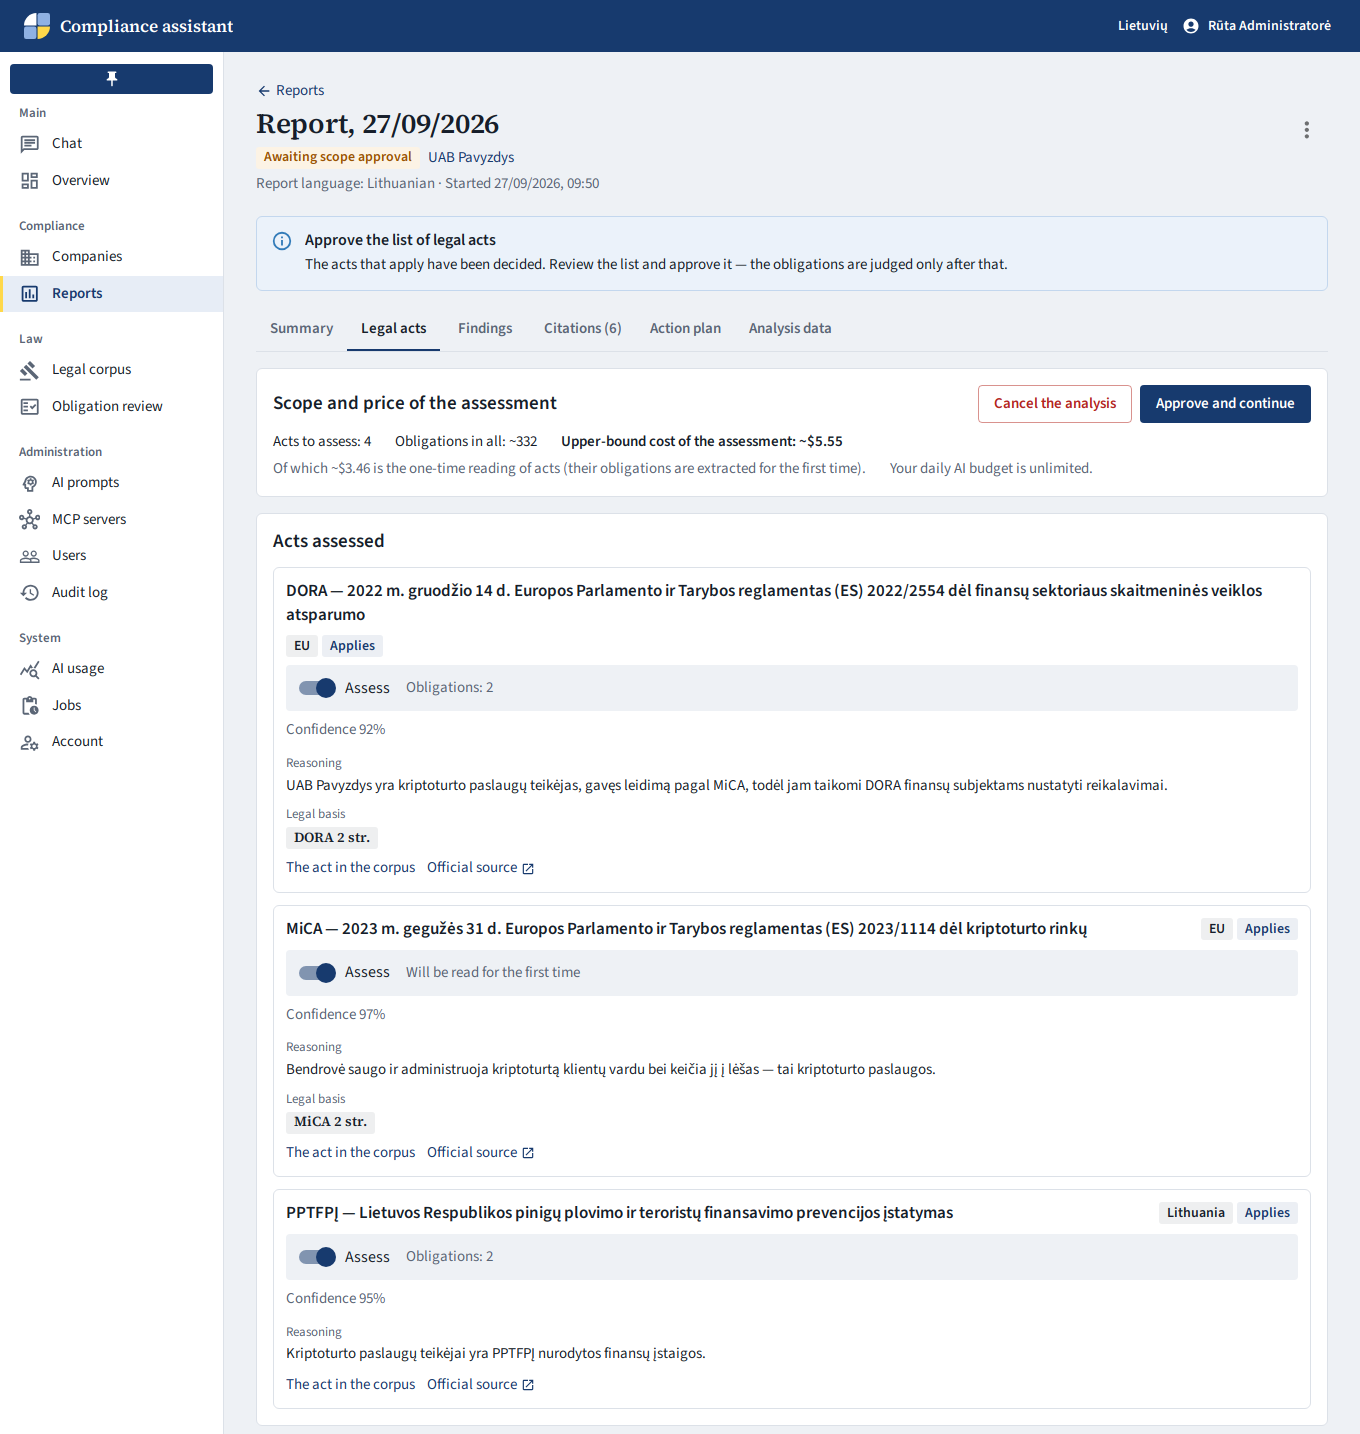
\includegraphics[width=.76\textwidth, trim=240 539 0 52, clip]{figures/screens/report-scope}
\caption{A report waiting for its scope approval. The banner says what is asked; the price
panel carries the two buttons; each act has its \ui{Assess} switch with the number of
obligations it would bring, or \enquote{Will be read for the first time} when its obligations
are still to be extracted.}\label{fig:console:scope}
\end{figure}

\paragraph{While it runs.} A queued or running report shows the progress card
(\file{pages/Reports/ReportProgress.jsx}): the steps of this run with their state and duration,
each finished step with its model and cost, the AI cost so far and the elapsed time.
\ui{Stabdyti analizę} (Stop the analysis) stops it at its next step; money already spent is not
returned. The steps are the job's, and a plain user sees only the jobs they started, so a report
an administrator started shows its progress line without the steps, and says why.

\paragraph{The finished report.} A finished report has six tabs (\code{TABS} in
\file{ReportDetail.jsx}): \ui{Santrauka} (Summary), \ui{Teisės aktai} (Legal acts),
\ui{Išvados} (Findings), \ui{Nuorodos} (Citations), \ui{Veiksmų planas} (Action plan) and
\ui{Analizės duomenys} (Analysis data, the company's profile as it was frozen for the run ---
after a scope review, as the second part of the run read it).
Above them stand the sign-off and, when an act the report used has a newer version since,
the warning \ui{Teisės aktai atnaujinti} (Legal acts updated) with \ui{Paleisti iš naujo} (Run
again).

\begin{figure}[htbp]
\centering
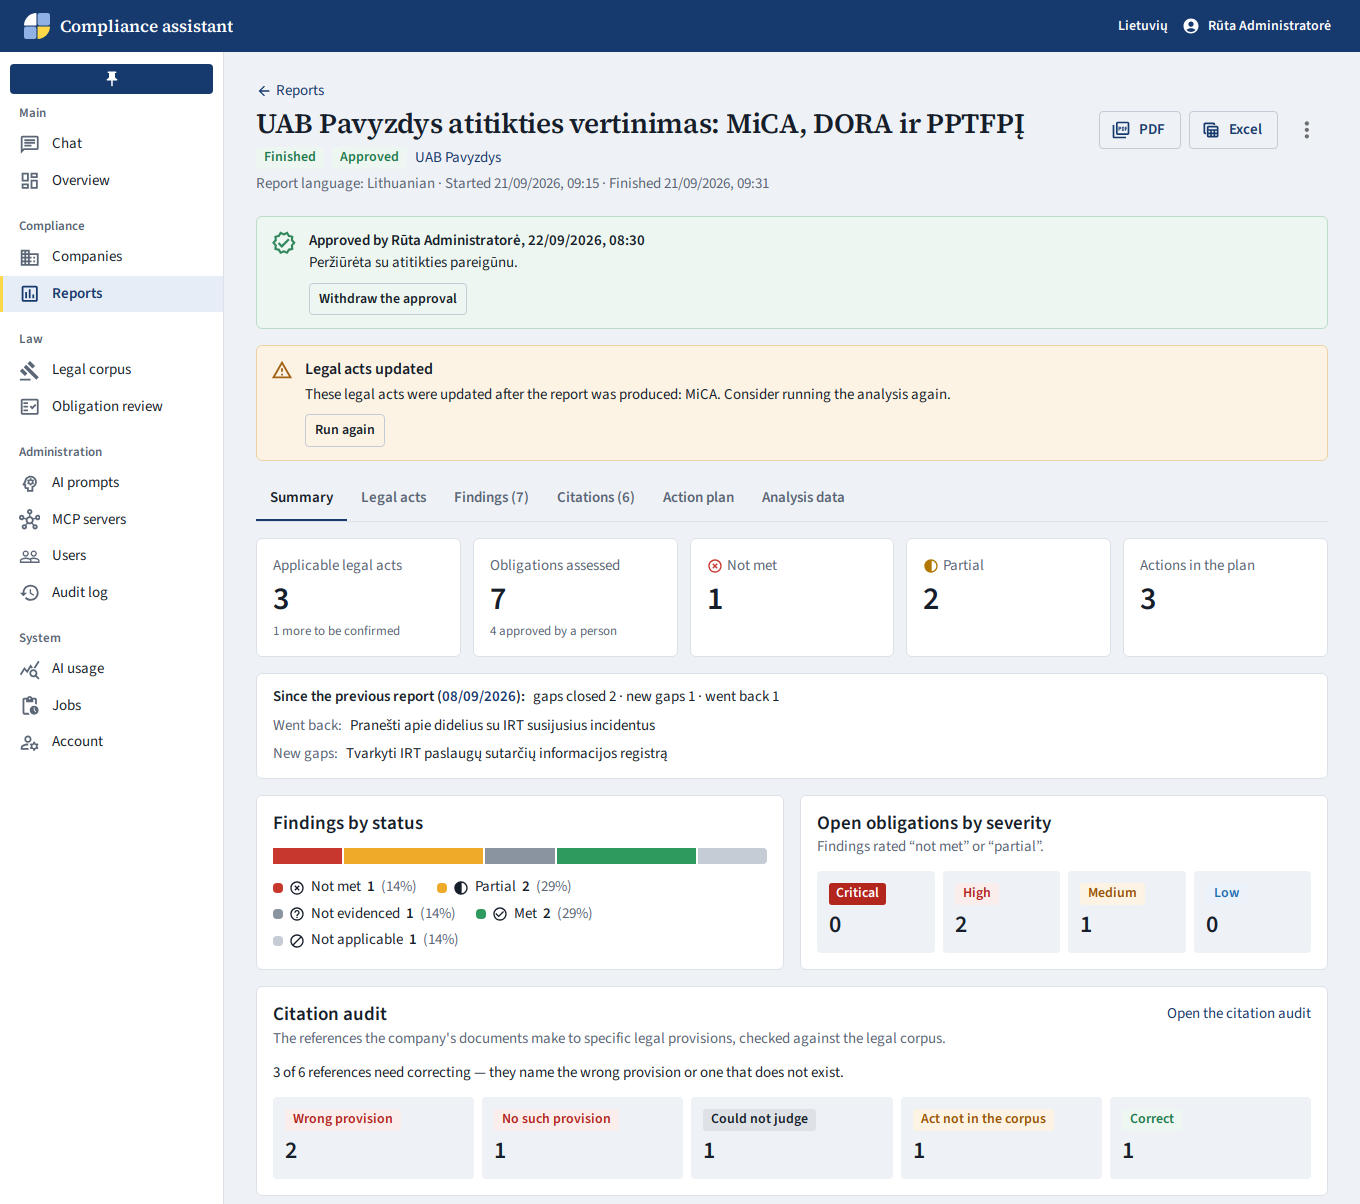
\includegraphics[width=.72\textwidth, trim=240 234 0 52, clip]{figures/screens/report-overview}
\caption{The summary tab of a finished, signed-off report. From the top: the approval banner
with \ui{Withdraw the approval}; the warning that an act was updated after the run; the tiles;
what moved since the previous report; the findings by status as one bar; the open obligations by
severity. The citation audit's counts follow below.}\label{fig:console:overview-report}
\end{figure}

The summary (\file{ReportOverview.jsx}, \cref{fig:console:overview-report}) is what a board
member reads first: the acts and obligations assessed and how many of those obligations a
person had approved, the counts of the five statuses, the open obligations by severity, what
changed since the company's previous report, the acts not assessed because their applicability
is still to be confirmed (with the way to their questions), the preparation for acts that apply
later, the citation audit's counts, the model's executive summary, and the provenance --- the
prompt versions, models and act versions that produced the report, and its AI cost. The counts
are today's result: they cover the acts in force for the company, follow a reviewer's override
where there is one, and leave out the company's own requirements, which are counted apart.

The acts tab (\file{ReportActs.jsx}) shows what the report did with each act --- assessed,
assessed as preparation for a later date, not assessed until a question is answered --- and,
folded, the directives, the acts that only organise an authority, those judged not to apply and
those the catalogue screened out. An act updated after the run is marked on its card.

\paragraph{Findings and the review dialog.} The findings tab (\file{ReportFindings.jsx}) groups
the findings by act or by domain, filters them by status and severity, and searches their text.
A card shows the status and severity chips, \ui{Peržiūrėta} (Reviewed) when a person overrode
the model, and \ui{Nepatvirtinta pareiga} (Unreviewed obligation) when the obligation itself was
never approved by a person (\cref{fig:console:finding}). Opened, it gives the obligation in the
act's words (set in the serif, as everything quoted from a source), the assessment, the cause
when a reviewer wrote one, the consequence --- the sanction ceilings the act provides, always
with the note that it is a ceiling and not a forecast --- the evidence with its quotations, the
recommendation and deadline, the reviewer's note, and the earlier verdicts on the same
obligation in the company's earlier reports. A quotation under the yellow marker opens the
document drawer at its place.

\begin{figure}[htbp]
\centering
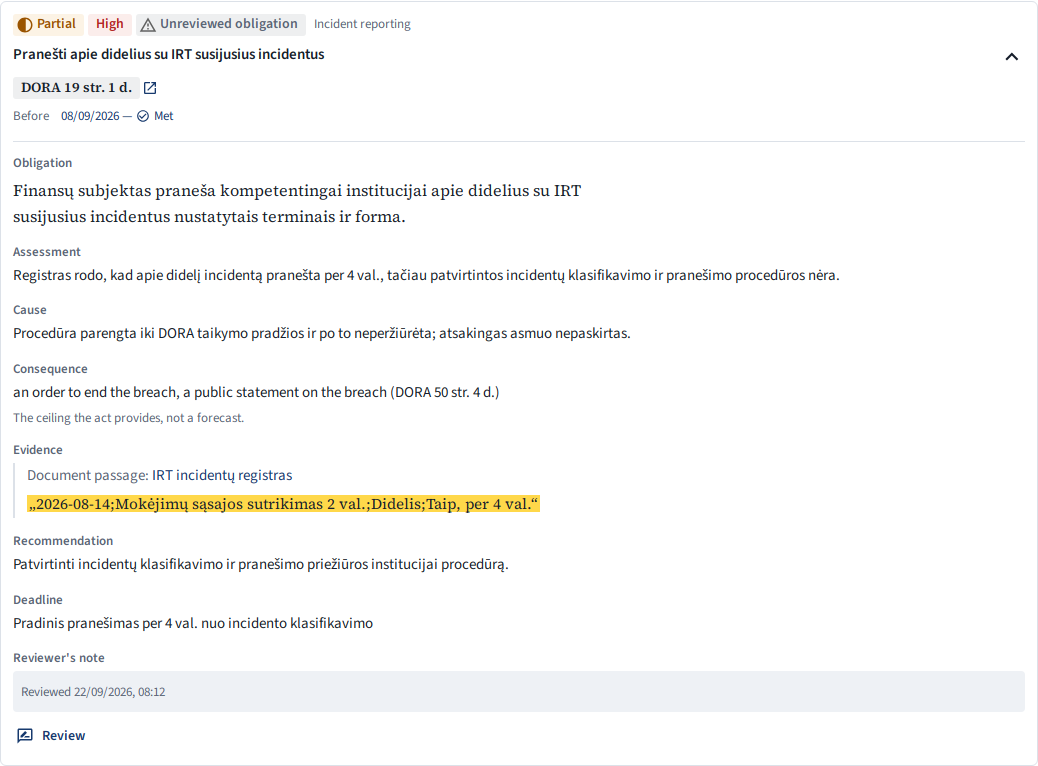
\includegraphics[width=.505\textwidth]{figures/screens/report-finding-card}\hfill
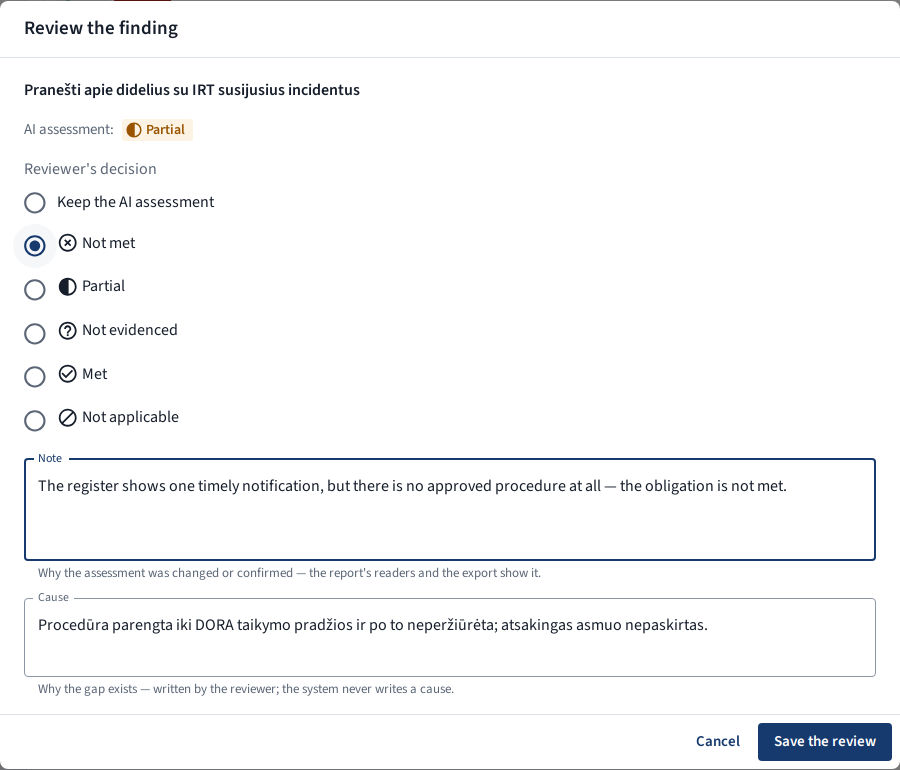
\includegraphics[width=.475\textwidth]{figures/screens/finding-review-dialog}
\caption{Left, one finding opened: the chips, the earlier verdict (\ui{Before}), the
obligation, the assessment, the cause, the consequence with its \enquote{ceiling, not a
forecast} note, the evidence passage under the yellow marker, and \ui{Review}. Right, the review
dialog: the AI assessment stays in view; the reviewer keeps it or picks another status, writes
the note, and writes the cause, which the system never writes.}\label{fig:console:finding}
\end{figure}

\ui{Peržiūrėti} (Review) opens the review dialog (\file{FindingReviewDialog.jsx}). The model's
verdict stays visible; the reviewer either keeps it (\ui{Palikti DI vertinimą}, Keep the AI
assessment) or picks another of the five statuses, and writes a note. The dialog also holds the
\ui{Priežastis} (Cause): why the gap exists. The cause is the one part of a finding only a
person writes --- the documents show what is missing, not why --- so neither the analysis nor
the chat assistant fills it. The dialog sends
\route{PATCH}{/api/reports/{id}/findings/{fid}}; the status every view and export then shows is
the override, and any review withdraws the report's sign-off on the server.

\paragraph{The citation audit.} The \ui{Nuorodos} (Citations) tab (\file{ReportCitations.jsx},
\cref{fig:console:citations}) lists every reference the company's documents make to a specific
provision, checked when the report ran (\cref{ch:company,ch:report}). Each card has the verdict
--- \ui{Teisinga} (Correct), \ui{Ne ta nuostata} (Wrong provision), \ui{Tokios nuostatos nėra}
(No such provision), \ui{Akto nėra bazėje} (Act not in the corpus) or \ui{Nepavyko įvertinti}
(Could not judge) --- the document, the reference as written with what the document claims it
covers, and for a provision that exists its real heading, the check's note, an excerpt and its
links. Problems come first; toggles with counts filter by verdict.

\begin{figure}[htbp]
\centering
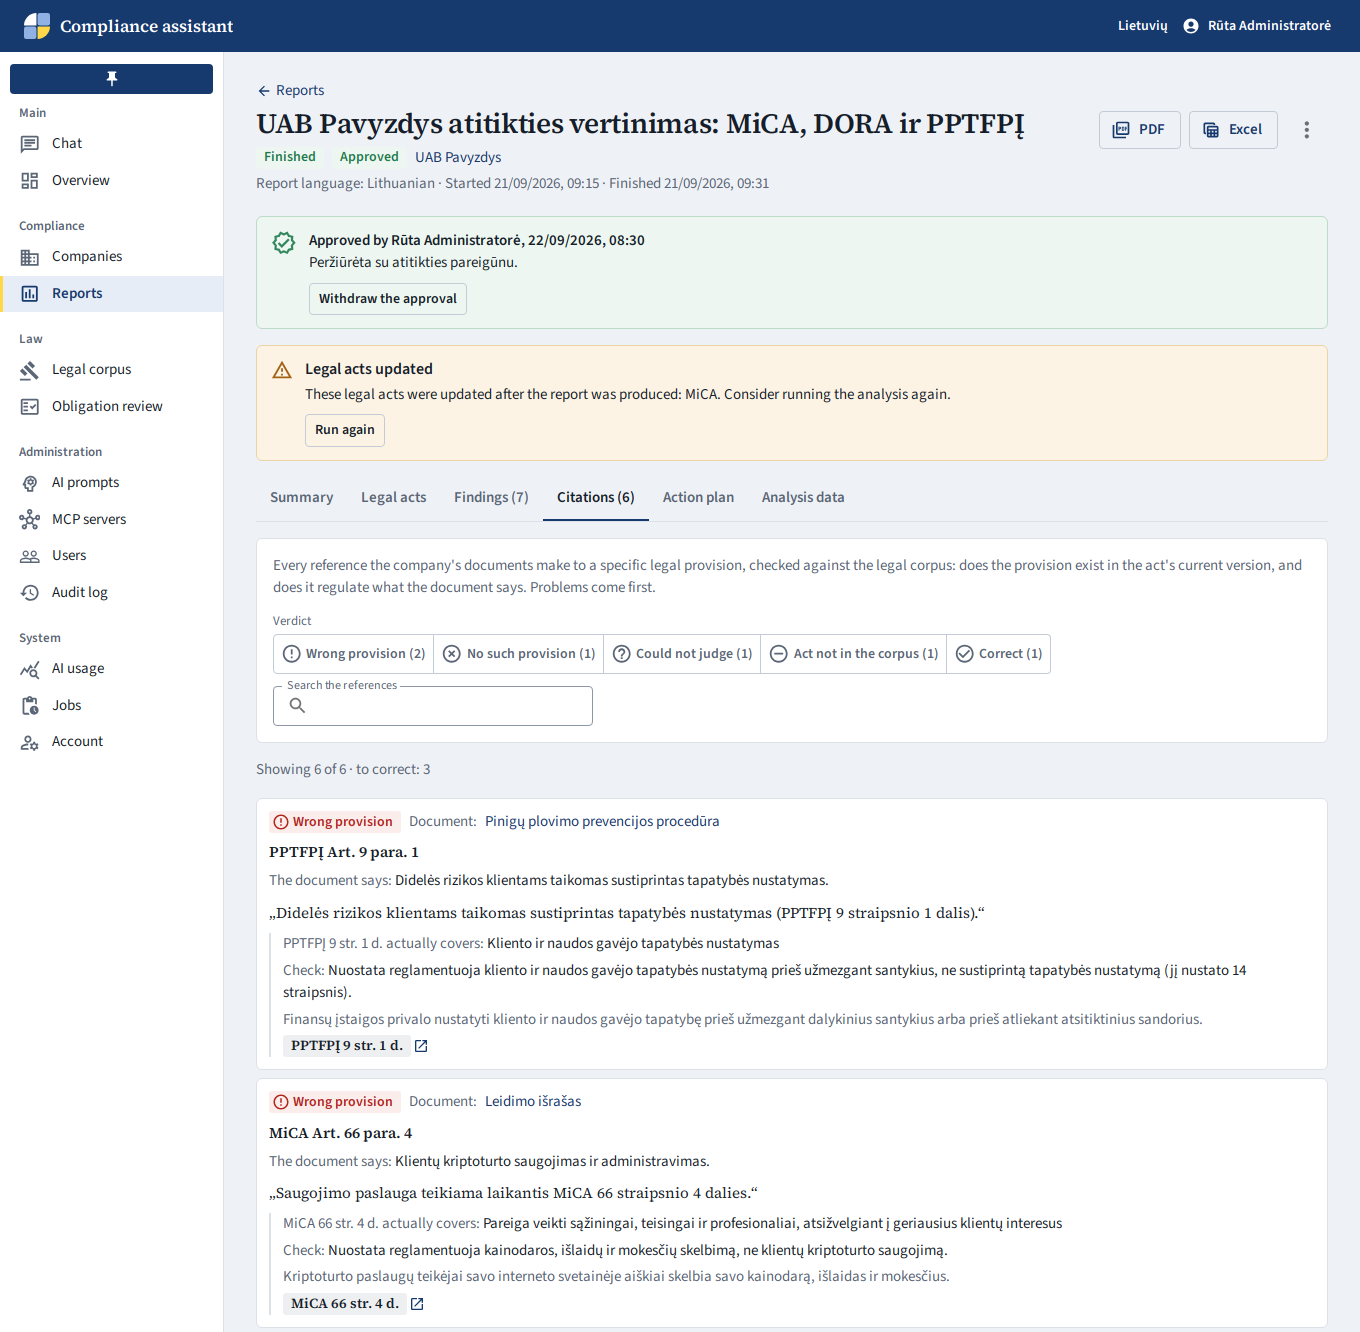
\includegraphics[width=.76\textwidth, trim=240 262 0 52, clip]{figures/screens/report-citations}
\caption{The citation audit of a report. Each card sets what the document says beside what the
cited provision actually covers, with the check's note and a link to the provision.}\label{fig:console:citations}
\end{figure}

\paragraph{The action plan.} The plan tab (\file{ReportActionPlan.jsx}) lists the actions in
order of priority, each with its description, timeframe, effort, owner and domain;
\ui{Susijusios išvados} (Related findings) opens the findings tab narrowed to the findings that
action closes. An action that only prepares for an act not yet in force is marked as preparation
and listed last.

\paragraph{Sign-off and exports.} \ui{Patvirtinti ataskaitą} (Approve the report) in the header
of a finished report opens a dialog that says what signing off means --- the person reviewed the
findings and the plan, and any later change to a finding withdraws the approval --- and takes an
optional note (\file{ReportApproval.jsx}, \route{PATCH}{/api/reports/{id}} with
\code{approved: true}). It also says that the sign-off moves the company's action register; the
notice that follows tells in words what moved (actions added, actions left out because one
already covers them, obligations confirmed met, earlier actions closed or sent back to work)
with a link to the register. A signed-off report shows a green banner with who approved it, when,
the note, and \ui{Atšaukti patvirtinimą} (Withdraw the approval). The header also carries the
exports, \ui{PDF} and \ui{Excel}, downloaded with the session's token
(\route{GET}{/api/reports/{id}/export?format=pdf|xlsx}); what the files hold is \cref{ch:report}.

\subsection{The action register and changes in the law}\label{sec:console:register}

\begin{figure}[htbp]
\centering
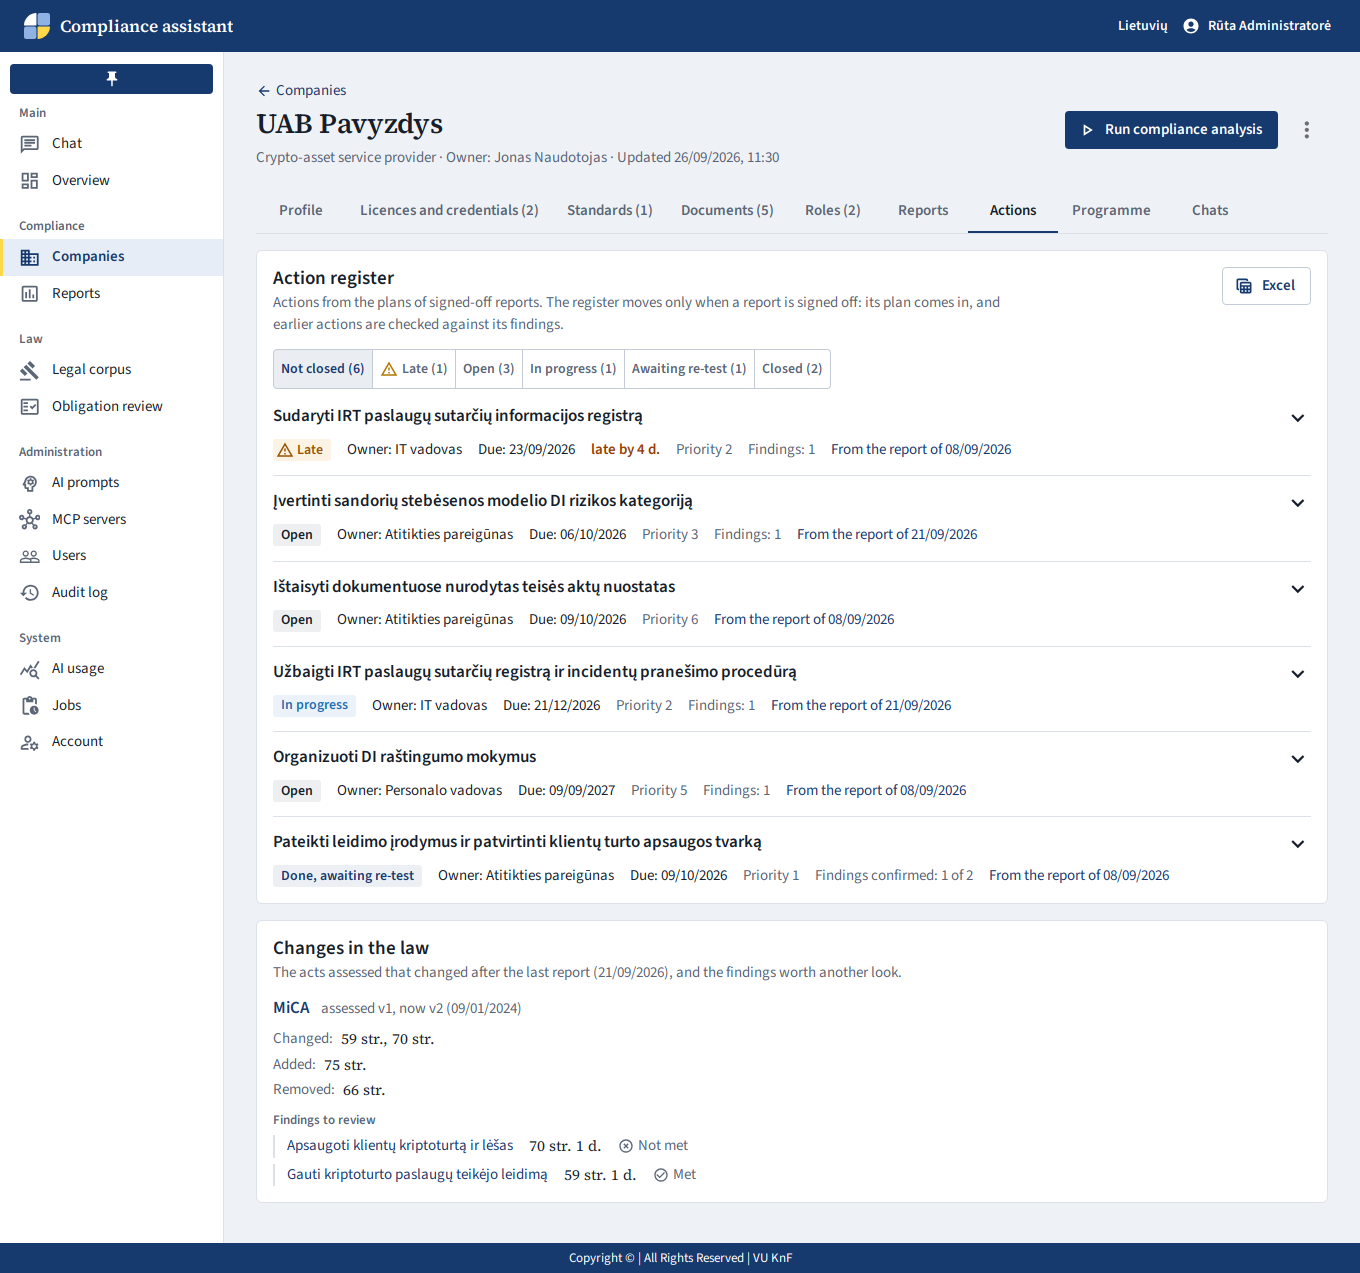
\includegraphics[width=.66\textwidth, trim=240 30 0 52, clip]{figures/screens/action-register}
\caption{A company's \ui{Actions} tab. The toggles count and filter the actions by state (the
late one with a warning mark, never by colour alone); each row gives the owner, due date,
priority, findings and the report it came from. Under the register, \ui{Changes in the law}: an
act that changed since the last report, its changed, added and removed provisions, and the
findings resting on them.}\label{fig:console:register}
\end{figure}

The \ui{Veiksmai} (Actions) tab of a company (\file{CompanyActions.jsx},
\cref{fig:console:register}) is the \term{action register}: what the plans of the company's
signed-off reports called for, kept after the reports. The card says under its title that the
register moves only when a report is signed off, because nothing on the tab adds an action. The
toggles count and filter the actions by state: \ui{Neuždaryti} (Not closed), \ui{Vėluoja} (Late),
\ui{Atviri} (Open), \ui{Vykdomi} (In progress), \ui{Laukia patikros} (Awaiting re-test) and
\ui{Uždaryti} (Closed). \enquote{Late} is not a state a person sets; it is shown for an open or
in-progress action whose due date has passed.

Opened, a row (\file{ActionRow.jsx}) lists the findings the action is to close, each marked
\enquote{confirmed} once a later signed-off report found its obligation met, and holds the form
a person keeps the action up with: owner, due date, status (open, in progress, done, closed) and
note, saved with \route{PATCH}{/api/actions/{id}}. \enquote{Done} is the owner's word and waits
for a later report to confirm it; closing by hand needs a note; an action a report closed cannot
be reopened here --- the closure is disputed at the finding, in that report. \ui{Excel} downloads
the register.

Under the register, \ui{Teisės aktų pokyčiai} (Changes in the law, \file{LawChanges.jsx}) shows,
for the company's latest finished report, every act it assessed that has a newer version now:
the version read and the version in force, the provisions changed, added or removed, and the
report's findings that rest on a changed or removed provision. The rules by which the register
moves are \cref{ch:register}.

\subsection{The compliance programme and its work products}\label{sec:console:programme}

\begin{figure}[htbp]
\centering
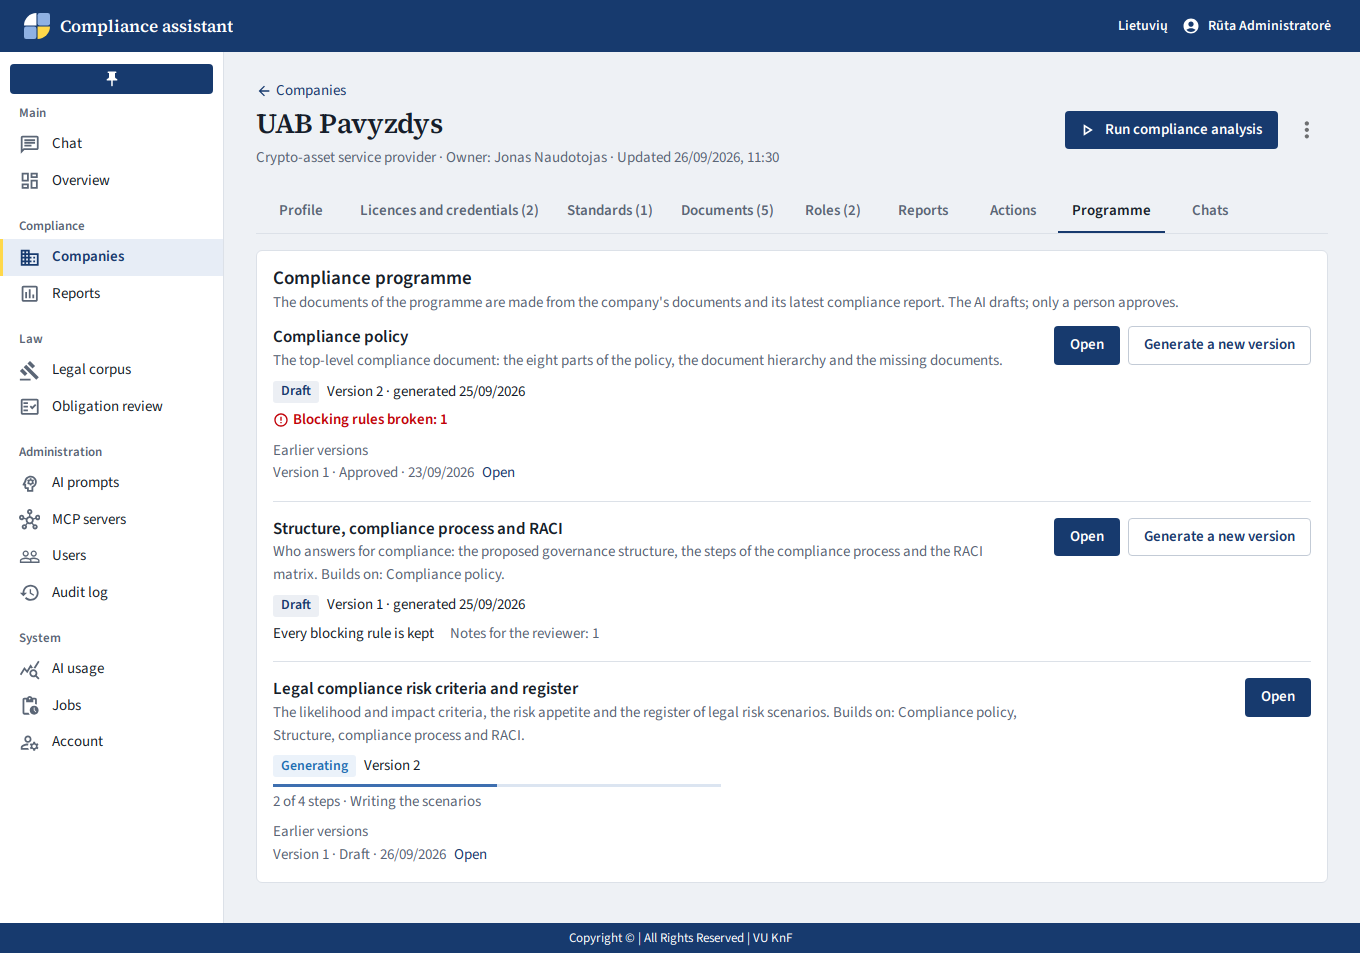
\includegraphics[width=.76\textwidth, trim=240 33 0 52, clip]{figures/screens/programme-tab}
\caption{A company's \ui{Programme} tab: the three kinds of work product in the order they build
on each other, where the newest version of each stands (a draft breaking one blocking rule, a
draft keeping them all, a version being generated with its step), the earlier versions, and the
buttons that fit the state.}\label{fig:console:programme}
\end{figure}

The \ui{Programa} (Programme) tab (\file{CompanyProgramme.jsx}, \cref{fig:console:programme})
lists the three kinds of \term{work product} the system drafts for a company, in the order each
builds on the ones before: \ui{Atitikties politika} (Compliance policy); \ui{Valdymo struktūra,
atitikties procesas ir RACI} (Structure, compliance process and RACI); and \ui{Teisinės atitikties
rizikos vertinimo kriterijai ir registras} (Legal compliance risk criteria and register). For
each it shows where the newest version stands --- not generated yet, queued or generating with
its step, a draft with the number of blocking rules it breaks, approved by whom and when, failed
or cancelled --- with the earlier versions under it. \ui{Generuoti} (Generate), or
\ui{Generuoti naują versiją} (Generate a new version), asks first: the dialog says that the
generation runs in the background for about five minutes and spends about \$0.50 of the day's AI
budget (\code{RUN_COST_USD}, the console's rounded copy of the API's figure), names the kinds it
builds on that do not exist yet, and takes the document's language.

\begin{figure}[htbp]
\centering
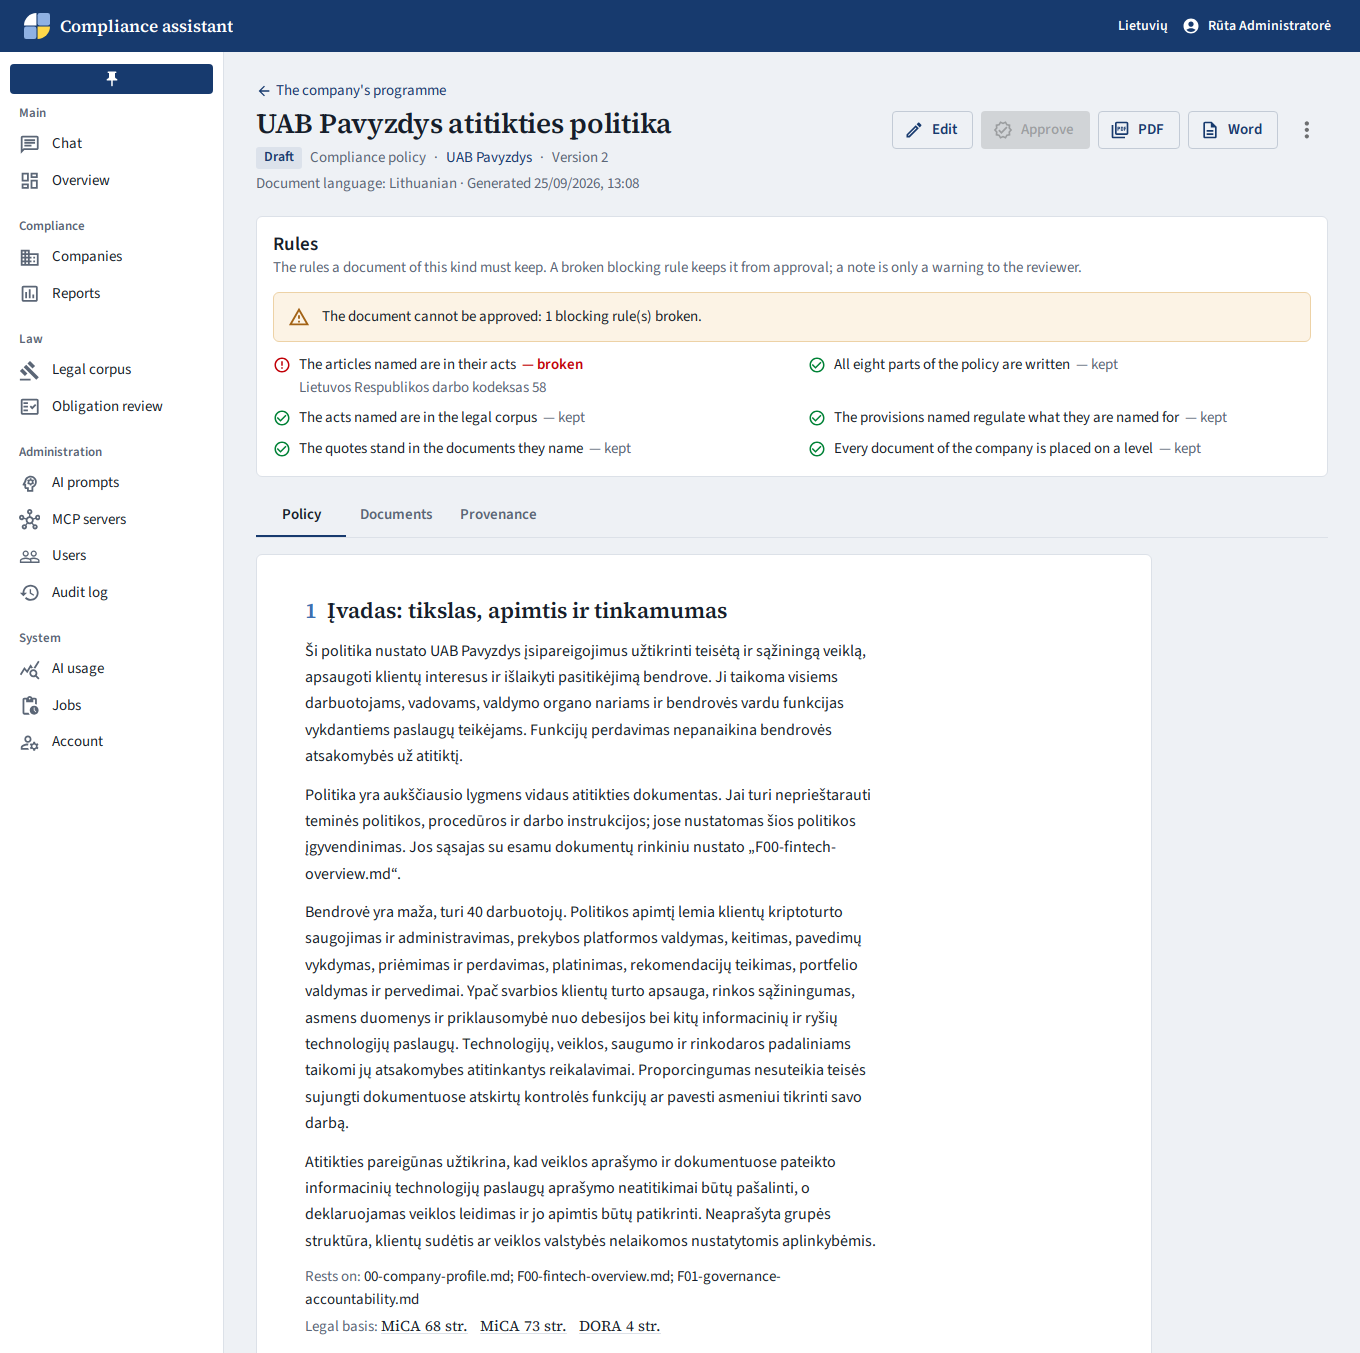
\includegraphics[width=.76\textwidth, trim=240 453 0 52, clip]{figures/screens/product-policy}
\caption{A draft compliance policy (\code{/console/programme/:productId}). \ui{Approve} is off,
because the \ui{Rules} panel shows one blocking rule broken (an article named that its act does
not have). Below, the policy's tabs and the start of its first part.}\label{fig:console:product}
\end{figure}

\ui{Atidaryti} (Open) leads to the page of one work product (\file{pages/Programme/ProductPage.jsx},
\cref{fig:console:product}). Its header names the status --- \ui{Generuojama} (Generating),
\ui{Projektas} (Draft), \ui{Patvirtinta} (Approved) --- the kind, the company and the version, and
carries the actions. Under it stands the \ui{Taisyklės} (Rules) panel (\file{RulesPanel.jsx}):
the backend checks every product against the rules of its kind, and the panel lists each rule as
kept or broken, a broken rule either blocking --- it keeps the product from approval --- or a note
for the reviewer, with the detail of what broke it. Below, the content in tabs that follow the
kind (\code{KIND_TABS} in \file{programmeUtils.js}), each kind ending with \ui{Kilmė}
(Provenance): what the product was made from, which prompts and models wrote it, and what the run
cost.

\begin{table}[H]
\caption{The tabs of a work product's page, by kind.}\label{tab:console:producttabs}
\begin{tabularx}{\textwidth}{@{}L{30mm}YL{30mm}@{}}
\toprule
\hd{Kind} & \hd{Tabs} & \hd{Exports} \\
\midrule
\code{policy} & \ui{Politika} (Policy), \ui{Dokumentai} (Documents), \ui{Kilmė} (Provenance) &
PDF, Word \\
\code{governance} & \ui{Struktūra} (Structure), \ui{Procesas ir RACI} (Process and RACI),
\ui{Pareigybės ir spragos} (Positions and gaps), \ui{Kilmė} & PDF \\
\code{risks} & \ui{Registras} (Register), \ui{Kriterijai} (Criteria), \ui{Kilmė} & PDF, Excel \\
\bottomrule
\end{tabularx}
\end{table}

\begin{figure}[htbp]
\centering
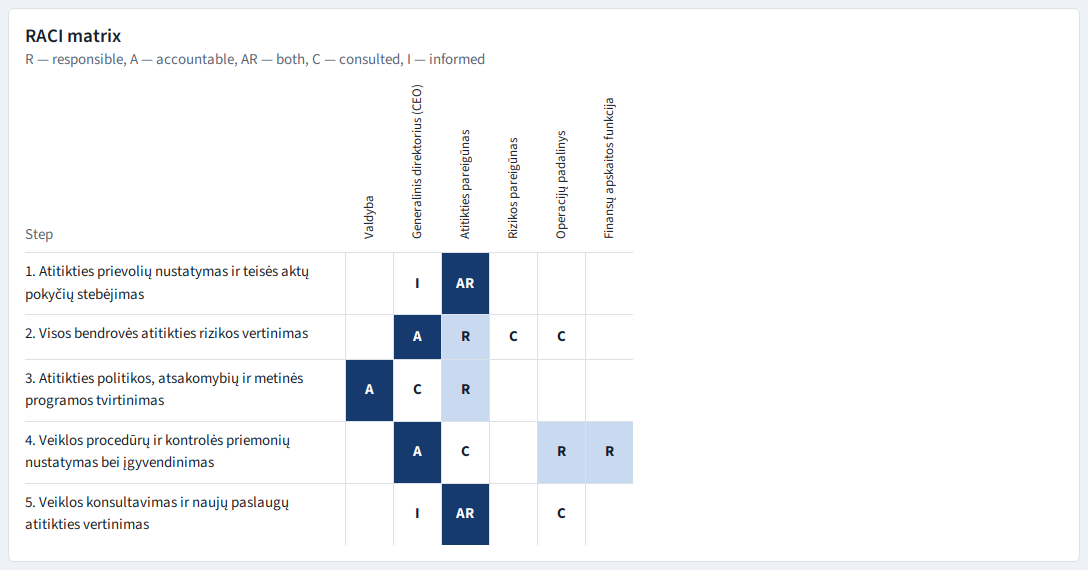
\includegraphics[width=.52\textwidth, trim=0 0 440 0, clip]{figures/screens/governance-raci}

\medskip
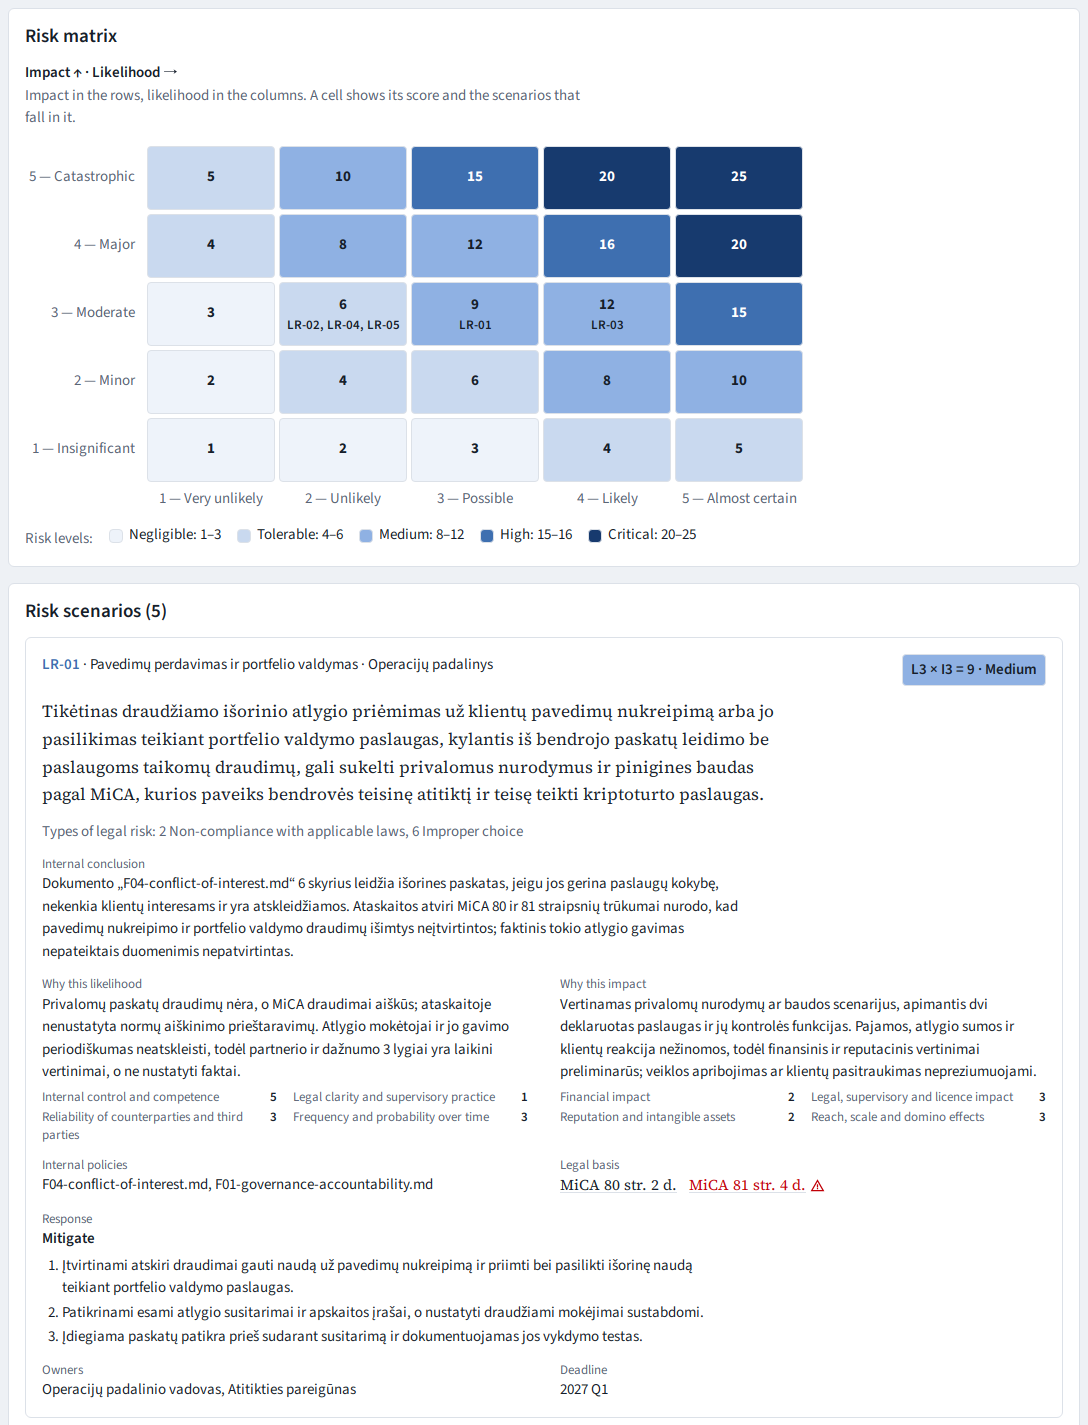
\includegraphics[width=.62\textwidth]{figures/screens/risk-register}
\caption{Two crops of work product pages. Above, the RACI matrix of a governance product: steps
in rows, roles in columns, every step with exactly one accountable role (A, or AR) and at least
one responsible (R). Below, the risk register: the 5×5 matrix with its five bands, and one
scenario with its eight dimension scores and the score \enquote{L3 × I3 = 9 · Medium}, which the
system computes; a cited provision it could not confirm carries a warning
mark.}\label{fig:console:productparts}
\end{figure}

\paragraph{Editing and approving.} \ui{Redaguoti} (Edit) turns a draft's content into forms:
the policy's parts, the documents' levels, the nodes of the structure, the steps of the process,
the RACI cells, the scenarios with their scores and plans, the criteria. The edits stay in the
page until \ui{Išsaugoti pakeitimus} (Save changes) sends the whole content
(\route{PUT}{/api/programme/{id}/content}) or \ui{Atmesti pakeitimus} (Discard changes) drops
them. The answer is the content as the server stored and checked it, and it replaces what is on
screen, so the rules panel then shows any rule the edit broke or mended. The page never works out
a score, a level or a band itself: a changed score is recomputed by the server on save. \ui{Patvirtinti} (Approve) is a person's act
(\file{ProductApproval.jsx}): it is off, with the reason, while a blocking rule is broken or
edits are unsaved, and it freezes the product --- an approved product cannot be withdrawn, only
copied by \ui{Nauja versija} (New version) into a new draft. The exports, one button per format
of the kind (\cref{tab:console:producttabs}), give a draft or an approved product as a file whose
cover says which it is. What the generation does and what the rules are is
\cref{ch:programme}.

\subsection{The legal corpus}\label{sec:console:corpus}

\ui{Teisės aktų bazė} (Legal corpus, \file{pages/Corpus/Corpus.jsx}) is open to every user,
since it is public law; an administrator also gets its write side. It has three tabs:

\begin{description}
  \item[\ui{Katalogas} (Catalogue)] The acts with their jurisdiction, type, whether in force,
    the current version and its ingestion status, the number of provisions, for an
    administrator the number of obligations, when the source was last checked and the last
    error. A plain user sees the enabled acts; an administrator all.
  \item[\ui{Paieška} (Search)] The same hybrid retrieval the chat assistant's search tool uses
    (\route{POST}{/api/corpus/search}), so a person can see what the assistant would be given
    for a
    question: each hit with its act, provision, score and passage (\cref{ch:corpus}).
  \item[\ui{Citatų tikrinimas} (Citation checker)] Up to 50 rows of act, article and optional
    paragraph, point and claimed topic (\route{POST}{/api/corpus/check-citations}). Each row
    says whether the provision exists in the act's current version, shows its real heading and
    opening, and --- when a topic is given --- whether it matches, which is a model call
    charged to the user's budget; the form says so.
\end{description}

\begin{figure}[htbp]
\centering
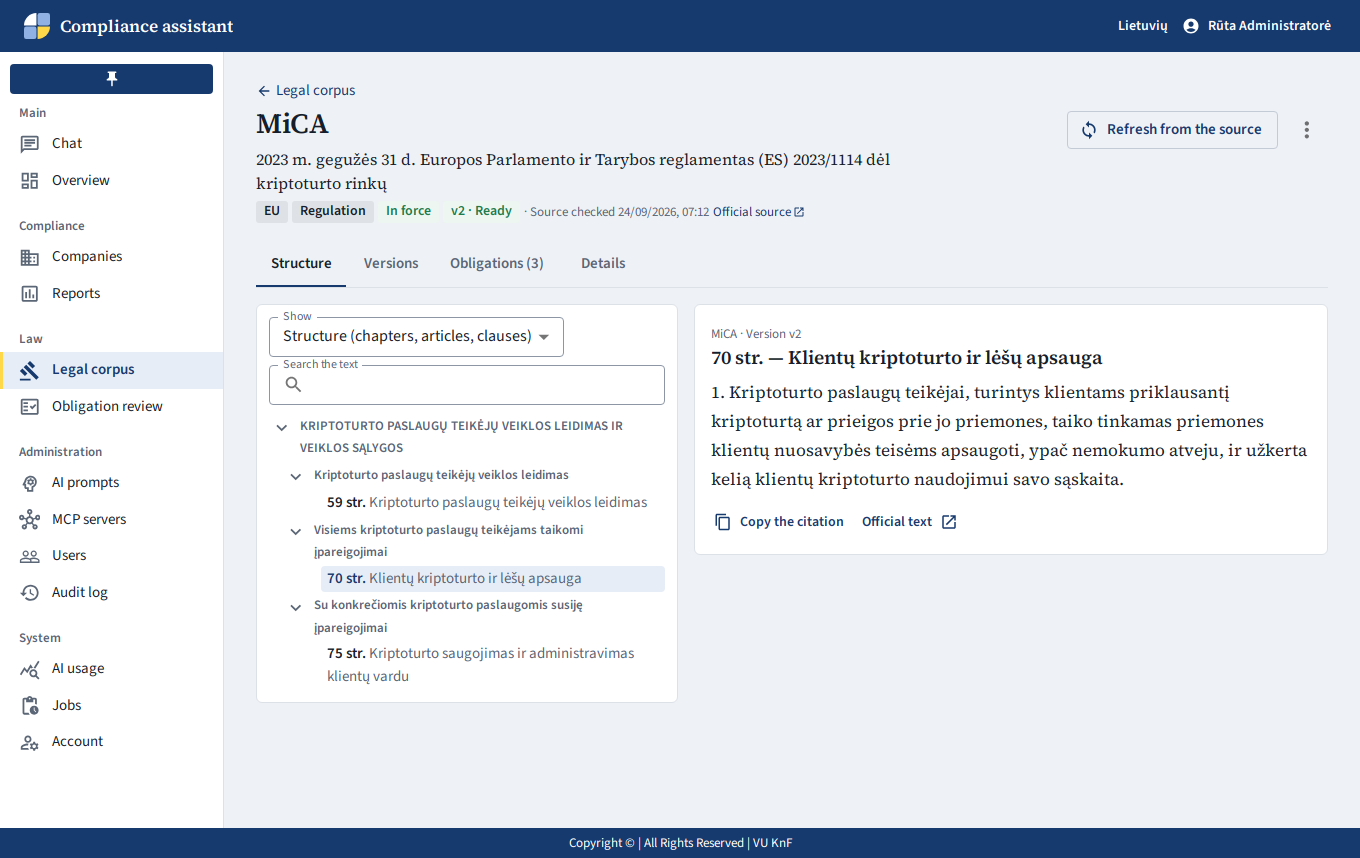
\includegraphics[width=.78\textwidth, trim=240 98 0 52, clip]{figures/screens/corpus-act}
\caption{One act of the corpus, structure tab: the provision tree with its filter and search,
and the chosen provision in the serif with \ui{Copy the citation} and \ui{Official text}. The
version chip and \ui{Refresh from the source} (an administrator's) are in the
header.}\label{fig:console:act}
\end{figure}

An act's page (\file{CorpusDocument.jsx}, \cref{fig:console:act}) has four tabs:
\ui{Struktūra} (Structure: the tree of chapters, articles and points beside the text of the
chosen provision, with its official link), \ui{Redakcijos} (Versions: every stored version with
its status, counts, parser and embedding model), \ui{Pareigos} (Obligations: the obligations
extracted from the act, read-only for a plain user) and \ui{Informacija} (Details: the
catalogue's record and, after it, what the models read from the act's own text --- whom it
covers and how many sanction tiers it lays down, each with the note the model left, or
\ui{Dar neskaityta}, not read yet). The chosen
provision is in the address (\code{?unit=}), which is how a report's citation links to it. An
administrator's actions sit in the header and its menu: \ui{Atnaujinti iš šaltinio} (Refresh
from the source), \ui{Apdoroti iš naujo (net jei nepasikeitė)} (Re-process, even if unchanged),
\ui{Įkelti naują redakciją} (Upload a new version, at most
60~MB), \ui{Išskirti pareigas} (Extract obligations), \ui{Patikrinti pareigas} (Check the
obligations, which queues the judge), \ui{Perskaičiuoti vektorius} (Re-embed),
\ui{Redaguoti metaduomenis} (Edit the metadata), \ui{Įjungti} / \ui{Išjungti} (Enable /
Disable) and \ui{Ištrinti teisės aktą} (Delete the legal act); for a standard also
\ui{Skaityti struktūrą kitaip} (Read the structure another way). Each costly or destructive one
is confirmed first. The catalogue's own header has \ui{Pridėti teisės aktą ar standartą} (Add
an act or standard), whose dialog asks for the source --- a CELEX number, an e-TAR identifier, a
page of the Bank of Lithuania, an address, or an uploaded file --- and the catalogue metadata;
its menu has the check of all sources and the re-embedding of everything. The machinery is
\cref{ch:corpus}.

\subsection{Obligation review}\label{sec:console:obligations}

\begin{figure}[htbp]
\centering
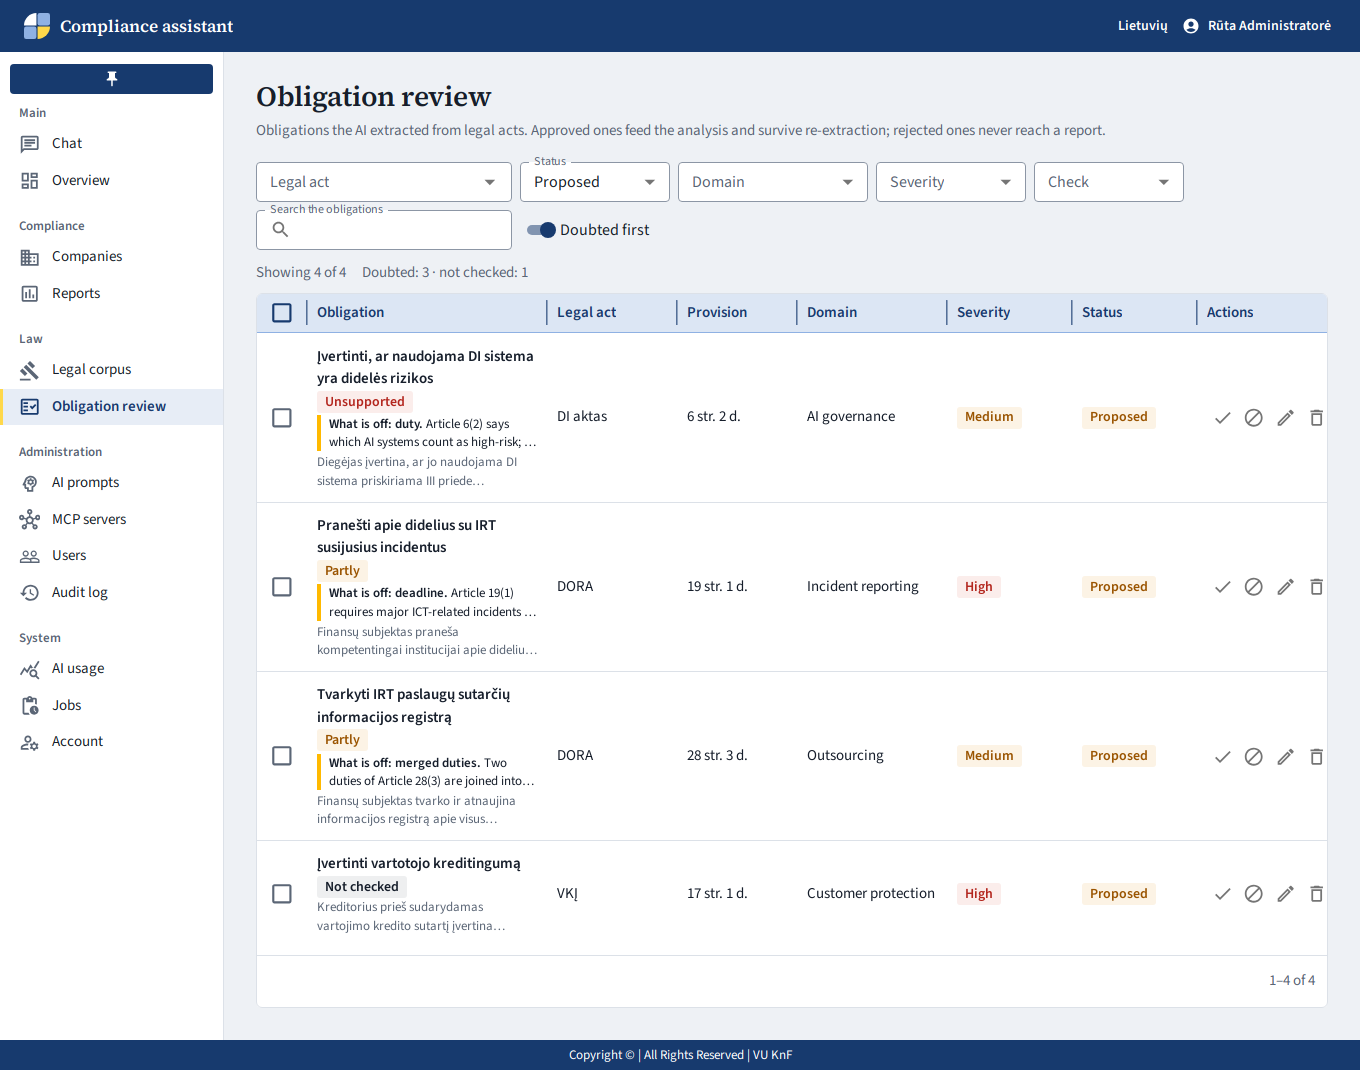
\includegraphics[width=.76\textwidth, trim=240 30 0 52, clip]{figures/screens/obligations}
\caption{The obligation review (\code{/console/obligations}), with \ui{Doubted first} on. Under
each title, the judge's verdict as a chip (\ui{Unsupported}, \ui{Partly}, \ui{Not checked}) and,
for a doubted one, what is off; on the right the row actions approve, reject, edit,
delete.}\label{fig:console:obligations}
\end{figure}

\ui{Pareigų peržiūra} (Obligation review, \file{pages/Obligations/ObligationsPanel.jsx},
\cref{fig:console:obligations}) is the administrator's queue of every obligation a model extracted
from the corpus. It opens on the proposed ones with \ui{Abejotinos pirmiausia} (Doubted first)
switched on: the obligations a second model call, the \term{judge}, doubted when it compared them with
the full text of the provisions they cite come first, because that is where a review starts. The
judge's verdict is a chip after the title --- quiet when it found the obligation supported or never
judged it, in the
attention tones for \ui{Iš dalies} (Partly) and \ui{Nepagrįstos} (Unsupported) --- with what is
off and the judge's note under a doubted row. The judge decides nothing. Filters narrow the list
by act, status, domain, severity and check. Rows are approved, rejected or edited one by one, or
selected and handled together with \ui{Patvirtinti pažymėtas} (Approve selected),
\ui{Atmesti pažymėtas} (Reject selected) or \ui{Grąžinti į pasiūlytas} (Set back to proposed);
a large selection goes to the server in chunks of 500. A row's title opens the edit dialog,
which shows the judge's verdict in full above the form; a changed title or text clears that
verdict. The same panel, read-only, is the obligations tab of an act for a plain user. The
extraction, the judge and the review are \cref{ch:obligations}.

\subsection{AI prompts}\label{sec:console:prompts}

\ui{DI instrukcijos} (AI prompts, \file{pages/Prompts/Prompts.jsx}) lists every stored prompt of
the chat and of the pipelines with its active version and model; a badge,
\ui{Laukia nauja numatytoji} (New default waiting), marks a prompt for which a deployment shipped
a newer default that is not active because an administrator's own version is.

\begin{figure}[htbp]
\centering
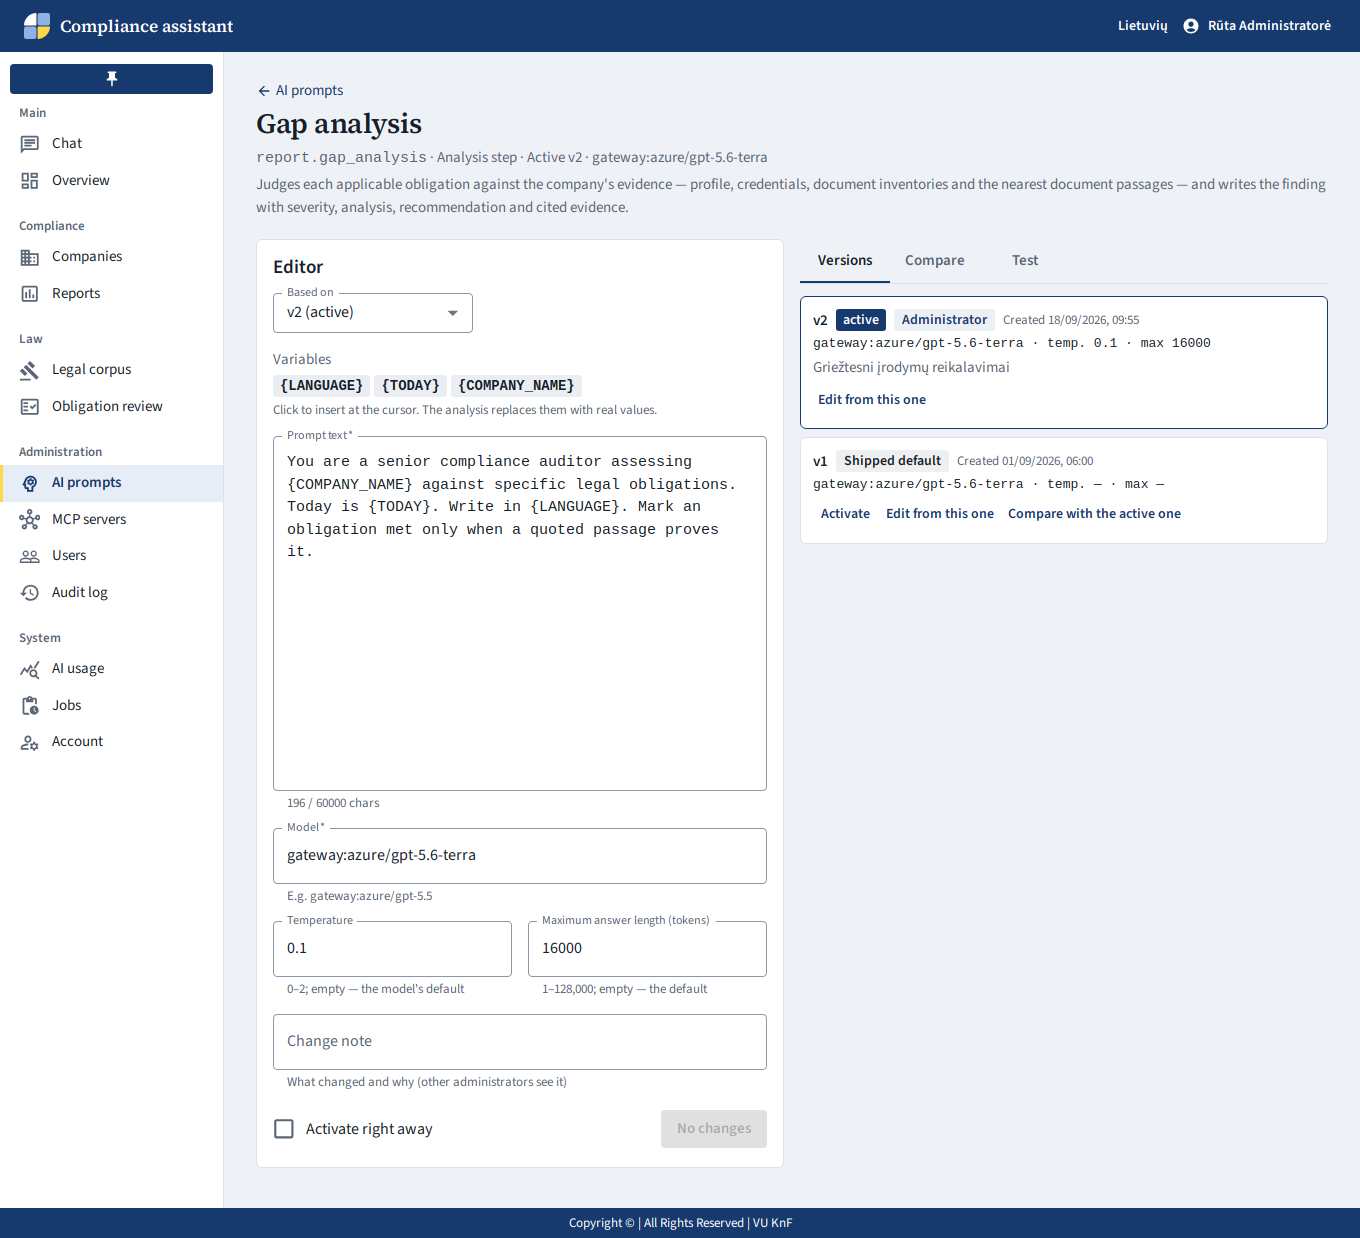
\includegraphics[width=.70\textwidth, trim=240 68 0 52, clip]{figures/screens/prompt-editor}
\caption{The prompt editor. On the left the draft: the version it starts from, the variables
(a click inserts one at the cursor), the text, the model, temperature, maximum answer length, a
change note and \ui{Activate right away}. On the right the \ui{Versions}, \ui{Compare} and
\ui{Test} tabs; the history marks the active version and the shipped default.}\label{fig:console:prompt}
\end{figure}

The editor (\file{PromptEditor.jsx}, \cref{fig:console:prompt}) holds a draft started from a
stored version. Saving never overwrites a version: it appends a new one
(\ui{Išsaugoti kaip naują versiją}, Save as a new version), and activates it at once only when
\ui{Iš karto aktyvuoti} (Activate right away) is ticked. Beside the draft are three tabs:
\ui{Versijos} (Versions: activate any version after a confirmation, load it into the editor, or
compare it with the active one), \ui{Palyginimas} (Compare: a line diff of any two versions or
the draft, with the settings compared above the text) and \ui{Bandymas} (Test: one model run of
the draft or a version on a given input, showing the answer, the tokens, the cost and the final
instructions the model got). A test costs money and the panel says so; it is charged to the
administrator's budget. The prompt store and its rules are \cref{ch:prompts}.

\subsection{MCP servers}\label{sec:console:mcp}

\ui{MCP serveriai} (MCP servers, \file{pages/Mcp/McpServers.jsx}) lists the external tool servers
whose tools the chat assistant may use, one card each: name, description, address, transport,
on or off, the names of its headers (their values are secrets and never come back), the allowed
tools and the tools the last test found. A new server is created switched off;
\ui{Tikrinti ryšį} (Test the connection) connects and lists its tools, which may take up to about
45 seconds, and only then is it switched on. The dialog checks the address the way the API does
--- \code{https} on the standard port to a public name, no IP address, no internal name, no user
and password --- because the assistant that connects to it sits next to every internal service
(\cref{ch:security}). A note on the page reminds the administrator that the server's host must also
be allowed by the outbound network rules (\cref{ch:ops}).

\subsection{Jobs}\label{sec:console:jobs}

\ui{Užduotys} (Jobs, \file{pages/Jobs/Jobs.jsx}) is the queue: the user's jobs, an
administrator's all, filtered by kind and status. The rows come in the order of the work ---
what runs now, then what waits in the order the worker will take it, then what ended --- and the
line above the table says how many run and wait. \ui{Atšaukti užduotį} (Cancel the job) cancels a
waiting job at once and stops a running one at its next step. \ui{Užduoties informacija} (Job
details) opens a drawer with the job's times, attempts, its AI cost in calls, tokens and dollars,
its error, its steps and its result; each finished step names the prompt version that ran it
(for instance \code{report.summary v3}), its models and calls. The jobs and the worker are
\cref{ch:arch}.

\subsection{AI usage}\label{sec:console:usage}

\begin{figure}[htbp]
\centering
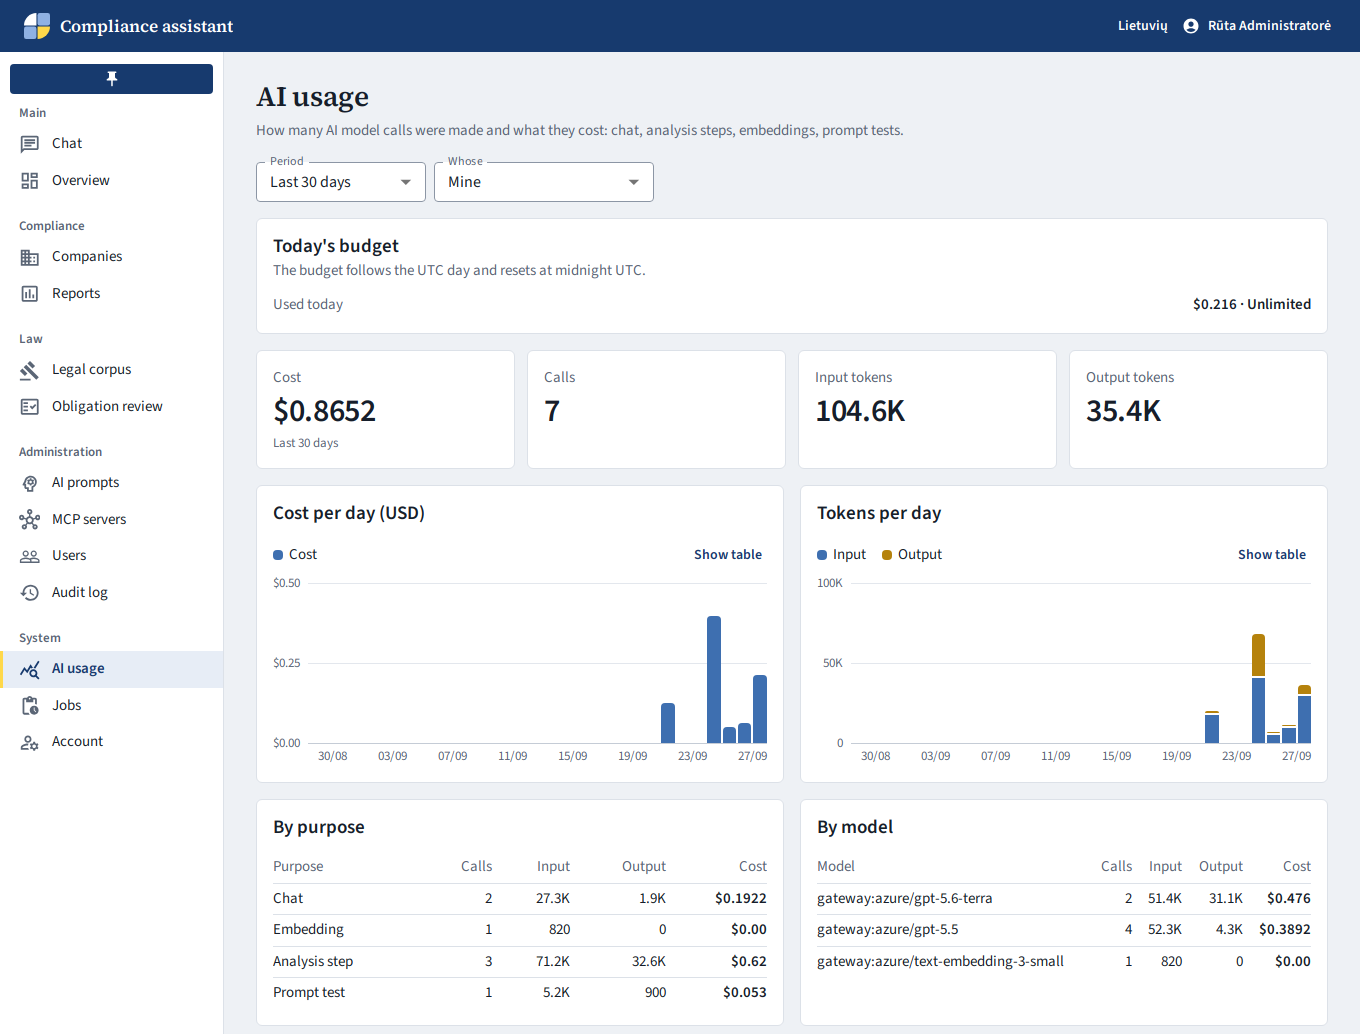
\includegraphics[width=.74\textwidth, trim=240 0 0 52, clip]{figures/screens/usage}
\caption{\ui{AI usage} for one user over 30 days: today's budget, the period's totals, cost and
tokens per day as two separate charts, and the splits by purpose and by model. The call log
follows below the splits.}\label{fig:console:usage}
\end{figure}

\ui{DI sąnaudos} (AI usage, \file{pages/Usage/Usage.jsx}, \cref{fig:console:usage}) shows what the
models cost. It leads with today's budget as a meter (the budget follows the UTC day), then the
chosen period's totals (7, 30 or 90 days: cost, calls, input and output tokens), the cost per day
and the tokens per day as two column charts --- two measures, two charts, never two axes --- and
the splits by purpose (\ui{Pokalbis} chat, \ui{Analizės etapas} analysis step,
\ui{Vektorizavimas} embedding, \ui{Instrukcijos bandymas} prompt test), by model and, for an
administrator looking at everyone, by user. \ui{Iškvietimų žurnalas} (Call log) lists every call;
one opens with its tool calls and, for a chat turn, the transcript --- the question and the
answer. Every user sees their own usage; an administrator can widen it to all accounts or look at
one, and so can read every user's chat transcripts here. That is stated to users in the user
guide and on the public site, and is \cref{ch:security}'s subject; the usage log and the budgets
are \cref{ch:models}.

\subsection{Audit log, users and account}\label{sec:console:admin}

\ui{Veiksmų žurnalas} (Audit log, \file{pages/Audit/Audit.jsx}) lists who changed what and when,
newest first, filtered by action (by area --- sign-in, users, companies, documents, legal acts,
obligations, reports, prompts, MCP servers, jobs --- or one action), by user and by an
\ui{Iki (imtinai)} (Until, inclusive) moment; \ui{Įkelti senesnius} (Load older entries) pages back
through the trail. An entry opens with its details.

\ui{Naudotojai} (Users, \file{pages/Users/Users.jsx}) is the administrator's directory:
\ui{Naujas naudotojas} (New user) with name, e-mail, role (\ui{Administratorius} or
\ui{Naudotojas}) and an initial password of at least 10 characters; editing the name, role,
whether the account is active, and \ui{Dienos DI biudžetas} (Daily AI budget), which is
\ui{Numatytasis} (Default, the installation's), \ui{Neribotas} (Unlimited) or \ui{Individualus}
(Custom, US dollars per UTC day); \ui{Keisti slaptažodį} (Reset password), which ends that user's
sessions; \ui{Deaktyvuoti} (Deactivate). \ui{Ištrinti su visais duomenimis} (Delete with all data)
has no dialog: the button must be held for two seconds (\file{components/LongPressButton/}), and
deletes the account with its companies, reports, documents and conversations. An administrator
cannot change their own role or state or delete themselves, and the last active administrator
cannot be demoted or deactivated; the controls say so before the API refuses.

\ui{Paskyra} (Account, \file{pages/Account/Account.jsx}) shows the user's name, e-mail and role,
changes the password (at least 10 characters and at most 72 bytes, which ends the other sessions)
and offers \ui{Atsijungti visuose įrenginiuose} (Log out everywhere).

\subsection{Controls that start a model call}\label{sec:console:modelbuttons}

\begin{table}[H]
\caption{The controls of the console that make the system call a model, with the chapter that
holds the call's path card and says who pays.}\label{tab:console:modelbuttons}
\begin{tabularx}{\textwidth}{@{}L{40mm}YL{28mm}@{}}
\toprule
\hd{Where} & \hd{Control} & \hd{Path card} \\
\midrule
Chat & sending a message; regenerating; the first message also names the conversation &
\cref{ch:chat} \\
Start dialog, scope screen & \ui{Pradėti analizę} (Start the analysis); \ui{Patvirtinti ir tęsti}
(Approve and continue) & \cref{ch:report,ch:obligations} \\
Company documents & an upload (the index's embeddings); the search over the documents (the query's
embedding) & \cref{ch:company} \\
Programme tab & \ui{Generuoti} / \ui{Generuoti naują versiją} & \cref{ch:programme} \\
Legal corpus & \ui{Paieška} (the query's embedding); \ui{Citatų tikrinimas} with a topic &
\cref{ch:corpus,ch:company} \\
One act (administrator) & \ui{Išskirti pareigas}; \ui{Patikrinti pareigas} (the judge);
\ui{Perskaičiuoti vektorius}; \ui{Atnaujinti iš šaltinio} or \ui{Įkelti naują redakciją} (the
new version's embeddings; for a standard, also the model that reads its structure) &
\cref{ch:corpus,ch:obligations} \\
Prompt editor (administrator) & \ui{Paleisti bandymą} (Run the test) & \cref{ch:prompts} \\
\bottomrule
\end{tabularx}
\end{table}

% ------------------------------------------------------------
\section{Where a person decides}\label{sec:console:decisions}

The system leaves a set of decisions to a person and never takes them itself. Each has one place
in the console and one control. \Cref{tab:console:decisions} gathers them; the chapters named
explain what each decision changes.

\begin{xltabular}{\textwidth}{@{}L{30mm}L{34mm}YL{18mm}@{}}
\caption{The decisions the console leaves to a person, the page that carries each, and the
control.}\label{tab:console:decisions}\\
\toprule
\hd{Decision} & \hd{Page} & \hd{Control and what it records} & \hd{Chapter} \\
\midrule
\endfirsthead
\toprule
\hd{Decision} & \hd{Page} & \hd{Control and what it records} & \hd{Chapter} \\
\midrule
\endhead
\bottomrule
\endlastfoot
Start a costly analysis & Start dialog (a company's page, the reports page) & \ui{Pradėti
analizę} after the upper-bound estimate and the remaining budget are shown. In the chat the
assistant shows the estimate and starts only on the user's explicit yes. & \cref{ch:report,ch:chat} \\
Approve the scope of a report & A waiting report, \ui{Teisės aktai} tab & An \ui{Vertinti} switch
per act, then \ui{Patvirtinti ir tęsti}; or \ui{Atšaukti analizę}. The report records who approved
the list and when, and the acts decided against the verdict. In the chat the assistant shows the
list and the price and continues only on the user's yes. & \cref{ch:report,ch:chat} \\
Approve an obligation & \ui{Pareigų peržiūra}; the edit dialog & The row's approve or reject
icon, or \ui{Patvirtinti pažymėtas} / \ui{Atmesti pažymėtas} / \ui{Grąžinti į pasiūlytas} for a
selection; edits in the dialog. The judge's verdict is shown and decides nothing. &
\cref{ch:obligations} \\
Override a finding, write its cause & A finished report, \ui{Išvados} tab & \ui{Peržiūrėti} opens
the dialog: keep the AI assessment or pick a status, a note, the \ui{Priežastis} (cause). Marked
\ui{Peržiūrėta}; withdraws the sign-off. & \cref{ch:report} \\
Sign a report off & A finished report, header & \ui{Patvirtinti ataskaitą} with an optional note;
\ui{Atšaukti patvirtinimą} withdraws it. Records who and when, and moves the action register. &
\cref{ch:register} \\
Keep an action up, close it by hand & A company's \ui{Veiksmai} tab, an opened row & Owner, due
date, status, note; closing by hand needs the note, which records why. & \cref{ch:register} \\
Verify a credential & A company's \ui{Leidimai ir licencijos} tab & \ui{Pažymėti patikrintu},
confirmed; records who and when. The gap analysis is told that a claimed licence is the
company's word: it may support \status{met} only with the caveat that it must be verified. In
the chat the assistant marks a credential verified only on the user's explicit word that it
was checked. &
\cref{ch:company,ch:chat} \\
Approve a work product & A work product's page, header & \ui{Patvirtinti}, off while a blocking
rule is broken or edits are unsaved; an optional note. Records who and when; freezes the product. &
\cref{ch:programme} \\
Activate a prompt version & The prompt editor & \ui{Aktyvuoti} on a version (confirmed),
\ui{Iš karto aktyvuoti} when saving, or \ui{Aktyvuoti} on a waiting shipped default. &
\cref{ch:prompts} \\
\end{xltabular}

\begin{humanbox}{What the console never does in a person's place}
No control of the console approves, signs off or activates without a person pressing it, and the
places where a model's result enters the record are marked as such: a finding a person overrode
says \ui{Peržiūrėta} and keeps the model's verdict in its tooltip; a finding whose obligation no
person approved says \ui{Nepatvirtinta pareiga}; a report run without the scope review says
\ui{Ataskaita paleista be aktų sąrašo peržiūros} (The report was run without a review of the list
of acts). The cause of a gap has no model behind it at all.
\end{humanbox}

% ------------------------------------------------------------
\section{The public site}\label{sec:console:site}

\begin{figure}[htbp]
\centering

\includegraphics[width=.70\textwidth]{figures/screens/site-home}
\caption{The public site's first page. The ink bar is the console's: the wordmark, the four
pages, the language switch and the way into the console --- \ui{Open the console} here, because
this browser holds a session; a visitor without one sees \ui{Sign in}. The hero shows the mark
as an object in three dimensions.}\label{fig:console:site}
\end{figure}

The public site (\file{site/}, \cref{fig:console:site}) is five pages under the same ink bar as
the console (\file{site/router.jsx}). It is plain React with the shared stylesheet, without the
component library. The way into the console in its bar reads \ui{Prisijungti} (Sign in), or
\ui{Atverti konsolę} (Open the console) when the browser already holds a session token
(\file{site/parts.jsx}). What the pages say about the analysis and the data follows the user
guide (\file{docs/markdown/lt/user-guide.md}), and the README asks that the two be changed together.

\begin{table}[H]
\caption{The pages of the public site.}\label{tab:console:sitepages}
\begin{tabularx}{\textwidth}{@{}L{34mm}Y@{}}
\toprule
\hd{Page} & \hd{What it says} \\
\midrule
\code{/} \ui{Atitikties spragų analizė finansų įstaigoms} (Compliance gap analysis for financial
institutions) & The claim, \enquote{Compliance is a mosaic. We show which pieces are missing.};
one finding up close with the passage of the company's document that decides it, marked; the
three things the assistant does (works out which acts apply, checks every duty against the
documents, draws up the action plan); the report; the conversation; where the texts come from
(the EU Publications Office, e-TAR, the Bank of Lithuania); and what the assistant does not do. \\
\code{/product} \ui{Produktas} (Product) & The way from a conversation to an approved report,
step by step: the conversation, the analysis with its cost known beforehand, a finding with its
evidence, the action plan, the check of the documents' own references, and review, approval and
the exports. \\
\code{/method} \ui{Metodika} (Method) & The six steps of an analysis; what a report does with an
act depending on how it applies; the five statuses and what severity means; what stays with a
person (review, approval, provenance); what the assistant does not do. \\
\code{/sources} \ui{Teisės aktai} (Legal acts) & How the texts are kept (split to the point,
checked weekly, linked to the official text) and the acts in the corpus by origin --- the EU's,
Lithuania's laws, the supervisors' --- then the licensing pages and the standards; the list says
it is the corpus as of November 2026 (\file{site/acts.js}, kept by hand in step with the
catalogue). \\
\code{/about} \ui{Apie} (About) & Where and for which course the product was made, who it is for,
how access works (accounts are made by an administrator), what happens to a user's data, how it
is built, and the caution that its findings are an aid. \\
\bottomrule
\end{tabularx}
\end{table}

The site shows the product rather than pictures of it: \file{site/specimens.jsx} redraws small
pieces of the console's screens --- a finding with its evidence, the status bar, the action plan,
a report's first page, a conversation, the reference check, an analysis at work --- as real text
in the visitor's language, with made-up content and the console's own labels, so the site cannot
call a status by another name than the product does. The home page and the method page end with
the same three limits (\file{site/Limits.jsx}): the assistant does not replace a lawyer, does not
assess practice, and does not guess. The pages move as they are read; under the browser's
reduced-motion setting the parts stand still in their final place. The site's \file{robots.txt} still keeps search engines out of the whole
origin.

% ------------------------------------------------------------
\section{How the console is built}\label{sec:console:built}

\paragraph{Libraries.} The console is a React~19 application built with Vite~7. Its components are
MUI~7 (with the MUI~X data grid for tables) styled together with Tailwind~4; the chat is built on
assistant-ui with the AI SDK's transport. Routing is React Router~7, with the routes in
\file{router.jsx} under the base \code{/console} and each page a module loaded on its first visit.
Data is fetched with axios through one client and cached by TanStack Query (\cref{sec:console:data}).
The versions are those in \file{vite/app/package.json}. The production image builds the files and
serves them as static files; there is no server-side rendering.

\paragraph{Shared pieces.} One data table (\file{components/DataTable/DataTable.jsx}), one
dialog (\file{components/UniversalModal/UniversalModal.jsx}), one status chip whose words carry
the state and whose colour only repeats it (\file{components/StatusChip/StatusChip.jsx}) and one
drop zone that refuses an unreadable or oversized file before sending it
(\file{components/FileDrop/FileDrop.jsx}) keep the pages alike.

\paragraph{Two languages kept in step.} The words live in \file{messages/}, one Lithuanian and one
English file per page, component and set of labels; \file{i18n.jsx} looks a key up, and a missing
key would show its dotted name on the screen, because the runtime falls back from one language to
the other only as a whole, never key by key. A guard, \file{vite/app/scripts/check-messages.js},
runs before every lint and every build and fails on a key present in one language and not the
other, on placeholders that differ between the two, on an English string identical to its
Lithuanian one (an untranslated string), and on a literal key in the code that resolves nowhere.
On 13 November 2026 it counted 2,824 keys in each language and verified 2,093 translation calls.

\paragraph{The look.} One light theme (\file{theme.js}) built from the brand's table. The colours
are those of the four-tile mark: ink (\texttt{\#173A6E}) for the top bar, buttons, links and the
focus ring; the mark's middle blue (\texttt{\#3E6FB0}) for the tint of the current place and for
progress; and its yellow (\texttt{\#FFD84A}) as the marker --- the highlighter of quoted evidence and of the text
selection, and the stripe of the current page in the navigation. The yellow never fills a control
or carries text. White sheets with hairline borders lie on a grey-blue canvas; only floating layers
cast a shadow; the status colours are kept for verdicts and states and always come with a label.
Two faces, self-hosted: Source Sans~3 for the interface and the assistant's answers, Source
Serif~4 for page titles and for everything quoted from a source --- provisions, obligations,
passages of the company's documents --- so a reader can always tell the source from the comment on
it. Everything is in sentence case. These are the faces and colours this document is set in.

\paragraph{Tests.} Every page, component and hook is tested with vitest in a simulated browser
against an in-process double of the backend that answers every endpoint the console calls; a
request no handler answers fails its test, and every page is tested as both roles and in both
languages. The suites and their counts are
\cref{ch:testing}.
